\documentclass[11pt,a4paper]{article}

% --- Paquetes Básicos ---
\usepackage{float}
\usepackage[utf8]{inputenc}
\usepackage[T1]{fontenc}
\usepackage[spanish,es-nodecimaldot]{babel}
\usepackage{geometry}
\geometry{margin=2.5cm}
\usepackage{graphicx}
\usepackage{titlesec}
\usepackage{booktabs}
\usepackage{hyperref}
\usepackage{setspace}
\usepackage{fancyhdr}
\usepackage{enumitem}
\usepackage{xcolor}
\usepackage{colortbl}
\usepackage{array}
\usepackage{longtable}
\usepackage{tikz}
\usepackage{pdflscape}
\usepackage{listings}

\usetikzlibrary{positioning,shapes.geometric,arrows.meta}

% --- Código SQL (listings) ---
\lstset{
  language=SQL, basicstyle=\ttfamily\footnotesize,
  keywordstyle=\color{blue}\bfseries, commentstyle=\color{gray}\itshape,
  stringstyle=\color{teal}, breaklines=true, breakatwhitespace=false,
  frame=single, columns=fullflexible, showstringspaces=false,
  numbers=left, numberstyle=\tiny\color{gray}, xleftmargin=1.5em,
  extendedchars=true, inputencoding=utf8,
  literate={á}{{\'a}}1 {é}{{\'e}}1 {í}{{\'i}}1 {ó}{{\'o}}1 {ú}{{\'u}}1
           {Á}{{\'A}}1 {É}{{\'E}}1 {Í}{{\'I}}1 {Ó}{{\'O}}1 {Ú}{{\'U}}1
           {ñ}{{\~n}}1 {Ñ}{{\~N}}1 {¿}{{?`}}1 {¡}{{!`}}1 {²}{{$^2$}}1
}

% --- Casilla por completar (mediciones propias) ---
\newcommand{\ph}{\textcolor{red}{\_\_\_\_}}

% --- Figura con captura: busca la imagen en varias carpetas y extensiones;
%     si no la encuentra, muestra un recuadro con el nombre esperado ---
\makeatletter
\newcommand{\captura}[2]{%
\begin{figure}[H]
\centering
\gdef\cap@found{}%
\@for\cap@dir:={imagenes/,./,Imagenes/,IMAGENES/,images/,imagenes/imagenes/}\do{%
  \@for\cap@ext:={png,jpg,jpeg,PNG,JPG,JPEG}\do{%
    \ifx\cap@found\@empty
      \IfFileExists{\cap@dir#1.\cap@ext}{\xdef\cap@found{\cap@dir#1.\cap@ext}}{}%
    \fi}}%
\ifx\cap@found\@empty
  \fbox{\parbox[c][3.5cm][c]{0.8\textwidth}{\centering Insertar captura:\\ \texttt{\detokenize{#1}}}}%
\else
  \includegraphics[width=\textwidth,height=0.4\textheight,keepaspectratio]{\cap@found}%
\fi
\caption{#2}
\end{figure}}
\makeatother

% --- Par de capturas (arbol + plan) de una consulta: {n}{escala archivo}{escala texto}{sin|con} ---
\newcommand{\planes}[4]{%
\captura{c#1_#2_#4_tree}{Query Plan Tree de la Consulta #1 con #3 datos #4 índices}
\captura{c#1_#2_#4_plan}{Query Plan de la Consulta #1 con #3 datos #4 índices}}

% --- Tabla de 5 ejecuciones por escala: \tablatiempos{consulta}{Sin|Con} ---
\newcommand{\tablatiempos}[2]{%
\begin{table}[H]
\centering
\small
\caption{Tiempos de ejecución --- Consulta #1 --- #2 índices}
\begin{tabular}{|c|r|r|r|r|}
\hline
\textbf{Ejecución} & \textbf{1k (ms)} & \textbf{10k (ms)} & \textbf{100k (ms)} & \textbf{1M (ms)} \\ \hline
1 & \ph & \ph & \ph & \ph \\ \hline
2 & \ph & \ph & \ph & \ph \\ \hline
3 & \ph & \ph & \ph & \ph \\ \hline
4 & \ph & \ph & \ph & \ph \\ \hline
5 & \ph & \ph & \ph & \ph \\ \hline
\textbf{Promedio} & \ph & \ph & \ph & \ph \\ \hline
\textbf{Desviación estándar} & \ph & \ph & \ph & \ph \\ \hline
\end{tabular}
\end{table}}

% --- Resultados de una consulta: 16 capturas y explicacion ---
\newcommand{\resultadoconsulta}[1]{%
\paragraph{Sin índices.}
\planes{#1}{1k}{1k}{sin}
\planes{#1}{10k}{10k}{sin}
\planes{#1}{100k}{100k}{sin}
\planes{#1}{1m}{1M}{sin}
\paragraph{Con índices.}
\planes{#1}{1k}{1k}{con}
\planes{#1}{10k}{10k}{con}
\planes{#1}{100k}{100k}{con}
\planes{#1}{1m}{1M}{con}
\paragraph{Explicación.}
}

% --- Configuración de Enlaces ---
\hypersetup{
    colorlinks=true,
    linkcolor=black,
    citecolor=black,
    urlcolor=blue
}

% --- Configuración de Encabezado y Pie ---
\pagestyle{fancy}
\fancyhf{}
\fancyhead[C]{Mantenimiento Predictivo de Turbinas Eólicas}
\renewcommand{\headrulewidth}{0.4pt}
\fancyfoot[L]{Grupo 11}
\fancyfoot[R]{\thepage}

% --- Configuración de Formato de Secciones ---
\titleformat{\section}{\normalfont\Large\bfseries}{\thesection.}{0.5em}{}
\titleformat{\subsection}{\normalfont\large\bfseries}{\thesubsection.}{0.5em}{}
\titleformat{\subsubsection}{\normalfont\normalsize\bfseries}{\thesubsubsection.}{0.5em}{}
\titleformat{\paragraph}{\normalfont\small\bfseries}{\theparagraph}{0.5em}{}
\titlespacing*{\paragraph}{0pt}{1ex}{0.5em}

\setstretch{1.2}
\setlength{\headheight}{14pt}

% ==========================================
%                CARÁTULA
% ==========================================
\title{
    \IfFileExists{UTEC.jpg}
    {
\includegraphics[width=10cm]{UTEC.jpg}\\[1cm]}
    {}
    \rule{\linewidth}{0.5mm}\\[0.4cm]
    \textbf{Proyecto Base de Datos I: Mantenimiento Predictivo de Turbinas Eólicas}\\
    \rule{\linewidth}{0.5mm}\\[0.3cm]
    \normalsize CS2041 Base de Datos I 
}

\author{
Alvaro David Pachas Chapeton\\
Guillermo Arturo Heredia Cadenas\\
Paul Ricardo Maguiña Quispe
}

\date{Ciclo 2026-2}

\begin{document}
\shorthandoff{<>}

\maketitle
\newpage

\renewcommand{\contentsname}{Índice General}
\tableofcontents
\newpage

% ==========================================
%           SECCIÓN 1: REQUISITOS
% ==========================================
\section{Requisitos}

\subsection{Introducción}

El mantenimiento de turbinas eólicas requiere conocer de manera continua el estado
de sus principales componentes mecánicos. Entre las variables utilizadas para esta
supervisión se encuentran las vibraciones generadas por elementos como rodamientos,
generadores y cajas multiplicadoras. Estas señales pueden presentar cambios antes de
que una falla sea visible, por lo que su almacenamiento histórico resulta útil para
identificar comportamientos anormales y planificar acciones de mantenimiento.

El presente proyecto propone una base de datos para un sistema de
\textbf{Mantenimiento Predictivo de Turbinas Eólicas}. La base de datos permitirá
administrar información de parques eólicos, turbinas, componentes, sensores de
vibración, lecturas históricas, alertas de mantenimiento, técnicos y órdenes de
trabajo. El objetivo es mantener la trazabilidad desde la medición producida por un
sensor hasta la intervención realizada sobre una turbina.

\subsection{Descripción general del problema/organización/empresa}

Para efectos del proyecto se considera una empresa operadora de parques eólicos que
administra múltiples turbinas instaladas en diferentes ubicaciones. Cada turbina
contiene componentes que requieren supervisión y puede disponer de uno o varios
sensores de vibración.

El principal problema se encuentra en la cantidad de información generada por los
sensores y en la dificultad de relacionar dicha información con las decisiones de
mantenimiento. Una misma turbina puede producir miles de mediciones durante un
periodo corto, mientras que las alertas y las órdenes de trabajo son registros menos
frecuentes pero indispensables para conocer qué ocurrió después de detectar una
anomalía.

Si las lecturas, alertas y órdenes de mantenimiento se encuentran en archivos o
sistemas separados, resulta difícil reconstruir el historial de una turbina. Por ello
se requiere una base de datos relacional que permita integrar estos elementos y
realizar consultas sobre el estado y comportamiento de los equipos.

\subsection{Necesidad/usos de la base de datos}

La implementación de una base de datos centralizada y normalizada responde a las
siguientes necesidades:

\begin{itemize}
    \item \textbf{Gestión de infraestructura eólica:}

    Registrar los parques eólicos administrados por la organización, las turbinas que
    pertenecen a cada parque y los componentes principales de cada turbina.

    \item \textbf{Monitoreo mediante sensores:}

    Registrar los sensores de vibración instalados en los componentes y almacenar las
    mediciones obtenidas a lo largo del tiempo.

    \item \textbf{Detección y seguimiento de anomalías:}

    Mantener un historial de alertas relacionadas con valores de vibración anormales,
    indicando su nivel de prioridad, estado y descripción.

    \item \textbf{Gestión del mantenimiento:}

    Crear órdenes de trabajo para inspecciones, mantenimiento preventivo o reparación
    de turbinas y asignarlas a un técnico responsable.

    \item \textbf{Trazabilidad:}

    Relacionar cada alerta con la lectura que la originó y con las órdenes de trabajo
    generadas para atenderla, permitiendo conocer qué acciones se realizaron frente a
    cada evento.

    \item \textbf{Análisis de datos:}

    Ejecutar consultas que permitan identificar turbinas con mayor cantidad de alertas,
    sensores con niveles altos de vibración y componentes con mantenimiento recurrente.

    \item \textbf{Escalabilidad:}

    Soportar grandes volúmenes de lecturas para realizar las pruebas de 1\,000,
    10\,000, 100\,000 y 1\,000\,000 de registros requeridas en el proyecto.
\end{itemize}

\subsection{¿Cómo resuelve el problema hoy?}

Para el escenario del proyecto se asume un modelo de trabajo parcialmente
fragmentado. Los sensores y sistemas de monitoreo generan archivos con mediciones,
mientras que las actividades de mantenimiento se registran por separado mediante
hojas de cálculo, reportes o aplicaciones internas.

Este funcionamiento permite conservar información básica, pero dificulta consultar
de forma integrada qué lectura produjo una alerta, qué componente se encontraba
afectado y qué mantenimiento fue realizado posteriormente.

\subsubsection{¿Cómo se almacenan/procesan los datos hoy?}

Se considera el siguiente escenario inicial:

\begin{itemize}
    \item Las lecturas de vibración son exportadas desde sistemas de monitoreo en
    archivos CSV u otros formatos tabulares.
    \item Los datos generales de parques, turbinas y componentes son almacenados en
    archivos administrativos.
    \item Las alertas pueden generarse en una plataforma de monitoreo o registrarse
    después de la revisión de las mediciones.
    \item Las órdenes de trabajo son administradas en hojas de cálculo o sistemas
    separados del sistema de monitoreo.
    \item Los técnicos actualizan manualmente el estado de las actividades asignadas.
\end{itemize}

La propuesta busca centralizar estos registros en PostgreSQL para mantener una única
fuente de información.

\subsubsection{Flujo de datos}

El flujo propuesto para el sistema es el siguiente:

\begin{enumerate}
    \item \textbf{Registro de infraestructura:} Se registran los parques eólicos,
    turbinas y componentes que serán monitoreados.

    \item \textbf{Instalación de sensores:} Cada sensor de vibración queda asociado al
    componente específico en el cual se encuentra instalado.

    \item \textbf{Captura de lecturas:} Los sensores generan mediciones de vibración
    que se almacenan con fecha y hora.

    \item \textbf{Análisis de condición:} Las lecturas son revisadas para identificar
    valores o patrones considerados anormales.

    \item \textbf{Generación de alerta:} Cuando una condición requiere atención se
    registra una alerta asociada al sensor correspondiente y, cuando es posible, a la
    lectura que la originó.

    \item \textbf{Evaluación de mantenimiento:} El supervisor revisa la alerta y
    decide si se necesita una intervención.

    \item \textbf{Creación de orden de trabajo:} Se registra una orden asociada a la
    turbina y se vincula con una o más alertas. Las órdenes preventivas o de
    inspección también pueden crearse sin una alerta previa.

    \item \textbf{Asignación técnica:} La orden se asigna a un técnico responsable.

    \item \textbf{Ejecución y cierre:} El técnico realiza la intervención y actualiza
    el estado de la orden hasta su finalización.
\end{enumerate}

\subsection{Descripción detallada del sistema}

\subsubsection{Objetos de información actuales}

Los objetos principales identificados para el sistema son:

\begin{itemize}
    \item \textbf{ParqueEolico:} Representa una instalación que agrupa múltiples
    turbinas eólicas.

    \item \textbf{Turbina:} Representa cada unidad de generación instalada dentro de
    un parque.

    \item \textbf{ComponenteTurbina:} Representa las partes de una turbina que se
    desea monitorear, por ejemplo generador, caja multiplicadora o rodamiento.

    \item \textbf{SensorVibracion:} Representa el dispositivo encargado de medir las
    vibraciones de un componente.

    \item \textbf{LecturaVibracion:} Almacena cada medición producida por un sensor
    junto con la fecha y hora en que fue registrada.

    \item \textbf{AlertaMantenimiento:} Representa una advertencia generada cuando el
    comportamiento observado requiere revisión.

    \item \textbf{OrdenTrabajo:} Registra una actividad de inspección, mantenimiento
    o reparación realizada sobre una turbina.

    \item \textbf{Tecnico:} Representa al trabajador responsable de ejecutar una orden
    de mantenimiento.
\end{itemize}

\subsubsection{Características y funcionalidades esperadas}

\begin{itemize}
    \item \textbf{Gestión de parques y turbinas:} Registrar y consultar la
    infraestructura administrada por la organización.

    \item \textbf{Gestión de componentes:} Identificar los componentes monitoreados
    dentro de cada turbina.

    \item \textbf{Gestión de sensores:} Registrar sensores, ubicación dentro del
    componente, modelo, unidad de medida y frecuencia de muestreo.

    \item \textbf{Registro masivo de lecturas:} Almacenar mediciones de vibración de
    manera continua o mediante cargas por lotes.

    \item \textbf{Generación de alertas:} Registrar eventos anormales indicando nivel,
    estado, descripción, valor detectado y la lectura que los originó.

    \item \textbf{Gestión de órdenes:} Registrar actividades de mantenimiento,
    prioridad, fechas, descripción y estado.

    \item \textbf{Asignación de responsables:} Asociar cada orden con el técnico que
    será responsable de su ejecución.

    \item \textbf{Trazabilidad lectura--alerta--orden:} Relacionar las lecturas con las
    alertas que producen y estas con las órdenes de trabajo utilizadas para atenderlas.

    \item \textbf{Historial de mantenimiento:} Consultar las alertas y órdenes
    relacionadas con una turbina durante un periodo determinado.
\end{itemize}

\subsubsection{Tipos de usuarios existentes/necesarios}

En primer lugar, se encuentran los \textbf{analistas de monitoreo}, encargados de
revisar las lecturas de los sensores y el comportamiento de las turbinas. Estos
usuarios requieren acceso principalmente a las mediciones históricas y a las alertas
generadas.

En segundo lugar, se encuentran los \textbf{supervisores de mantenimiento}, quienes
evalúan las alertas, crean órdenes de trabajo, establecen prioridades y asignan las
actividades al personal técnico.

Finalmente, se encuentran los \textbf{técnicos de mantenimiento}, responsables de
ejecutar las intervenciones sobre las turbinas y actualizar la información de las
órdenes asignadas.

También se considera un \textbf{administrador del sistema}, encargado de mantener
actualizados los datos maestros de parques, turbinas, componentes, sensores y
usuarios.

\subsubsection{Tipos de consulta, actualizaciones}

Entre las consultas de interés se consideran las siguientes:

\begin{itemize}[label={}, leftmargin=0cm, itemsep=0.3cm]
    \item ¿Qué turbinas poseen actualmente alertas de prioridad alta o crítica que
    todavía no han sido cerradas?

    \item ¿Cuál es el valor promedio, máximo y pico de vibración registrado por cada
    sensor durante un periodo determinado?

    \item ¿Qué sensores han superado un valor de vibración definido en varias
    mediciones consecutivas?

    \item ¿Qué componentes concentran la mayor cantidad de alertas de mantenimiento
    dentro de cada parque eólico?

    \item ¿Qué turbinas han generado la mayor cantidad de órdenes de trabajo durante
    un periodo determinado?

    \item ¿Cuántas órdenes pendientes o en proceso tiene asignadas cada técnico?

    \item ¿Cuál es el historial completo de alertas y órdenes de mantenimiento de una
    turbina específica?

    \item ¿Cuáles son los sensores con mayor frecuencia de alertas críticas en los
    últimos meses?
\end{itemize}

\paragraph{Carga y actualización de los datos.}
La forma en que se cargan y modifican los datos varía según el tipo de tabla. Las
lecturas de vibración son históricas: una vez registradas no se actualizan ni se
eliminan, solo se insertan nuevas mediciones.

\begin{table}[H]
\centering
\small
\caption{Forma de carga y frecuencia de modificación por tabla}
\label{tab:carga_datos}
\begin{tabular}{|p{4.2cm}|p{5.4cm}|p{4.8cm}|}
\hline
\textbf{Tabla(s)} & \textbf{Forma de carga} & \textbf{Frecuencia de modificación} \\ \hline
ParqueEolico, Turbina, ComponenteTurbina & Carga inicial única realizada por el administrador & Muy baja (altas o bajas de infraestructura) \\ \hline
SensorVibracion & Carga inicial y registro manual posterior & Baja (instalación, reemplazo o retiro) \\ \hline
Tecnico & Carga inicial y registro manual posterior & Baja (altas y bajas de personal) \\ \hline
LecturaVibracion & Carga por lotes desde archivos CSV del sistema de monitoreo & Muy alta (solo inserciones continuas) \\ \hline
AlertaMantenimiento & Generación por reglas de umbral o registro del analista & Media (cambios de estado durante la revisión) \\ \hline
OrdenTrabajo, AlertaOrden & Registro por el supervisor de mantenimiento & Media (cambios de estado hasta el cierre) \\ \hline
\end{tabular}
\end{table}

\paragraph{Tiempos de respuesta esperados.}
Los siguientes tiempos se plantean como objetivos de referencia para el escenario de
mayor carga (1\,000\,000 de lecturas) y serán contrastados con las mediciones
obtenidas en la etapa de experimentación.

\begin{table}[H]
\centering
\small
\caption{Tiempos de respuesta esperados para las operaciones más comunes}
\label{tab:tiempos_respuesta}
\begin{tabular}{|p{10.5cm}|c|}
\hline
\textbf{Operación} & \textbf{Tiempo esperado} \\ \hline
Registro o actualización de estado de una alerta u orden de trabajo & $<$ 0,5 s \\ \hline
Inserción de un lote de 1\,000 lecturas de vibración & $<$ 1 s \\ \hline
Consulta de alertas abiertas de prioridad alta o crítica por turbina & $<$ 1 s \\ \hline
Estadísticas de vibración (promedio, máximo, pico) de un sensor en un mes & $<$ 2 s \\ \hline
Historial completo de alertas y órdenes de una turbina & $<$ 2 s \\ \hline
Reportes agregados por parque o componente sobre toda la tabla de lecturas & $<$ 5 s \\ \hline
\end{tabular}
\end{table}

\subsubsection{Tamaño estimado de la base de datos}

Para esta estimación se considera únicamente el tamaño aproximado de los atributos y
no el overhead interno de PostgreSQL, páginas, índices o alineamiento de tuplas.
Los valores sirven como referencia para comparar el crecimiento relativo de las
tablas.

\par\bigskip

\begin{table}[H]
\centering
\small
\caption{Estimación simplificada de longitud de atributos por registro}
\label{tab:longitud_bytes_tablas}
\begin{tabular}{|l|l|r|}
\hline
\textbf{Nombre de la Tabla} & \textbf{Longitud estimada de atributos} & \textbf{Total aprox.} \\ \hline
ParqueEolico & 4 + 100 + 150 + 8 + 4 & 266 Bytes \\ \hline
Turbina & 4 + 4 + 30 + 60 + 60 + 8 + 4 + 20 & 190 Bytes \\ \hline
ComponenteTurbina & 4 + 4 + 60 + 40 + 60 + 20 & 188 Bytes \\ \hline
SensorVibracion & 4 + 4 + 30 + 50 + 20 + 8 + 4 + 20 & 140 Bytes \\ \hline
LecturaVibracion & 4 + 8 + 8 + 8 + 8 & 36 Bytes \\ \hline
AlertaMantenimiento & 8 + 4 + 8 + 8 + 15 + 50 + 8 + 255 + 20 & 376 Bytes \\ \hline
Tecnico & 4 + 100 + 60 + 100 + 15 & 279 Bytes \\ \hline
OrdenTrabajo & 8 + 4 + 4 + 8 + 8 + 8 + 15 + 50 + 255 + 20 & 380 Bytes \\ \hline
AlertaOrden & 8 + 8 & 16 Bytes \\ \hline
\end{tabular}
\end{table}

\paragraph{Pruebas de rendimiento y escalabilidad.}
Para la etapa de experimentación se generarán cuatro escenarios de carga:
1\,000, 10\,000, 100\,000 y 1\,000\,000 de registros. La entidad
\texttt{LecturaVibracion} será la principal tabla de crecimiento debido a que los
sensores generan datos con una frecuencia mucho mayor que las alertas y las órdenes
de trabajo. Estos escenarios permitirán analizar posteriormente los planes de
ejecución de consultas y comparar el comportamiento de la base de datos antes y
después de crear índices.

El Cuadro~\ref{tab:volumen_estimado} muestra el volumen esperado de cada tabla en el
escenario de mayor carga. La cantidad de registros de las tablas maestras es una
estimación de referencia y se mantendrá proporcional en los demás escenarios.

\begin{table}[H]
\centering
\small
\caption{Volumen estimado por tabla en el escenario de 1\,000\,000 de lecturas}
\label{tab:volumen_estimado}
\begin{tabular}{|l|r|r|}
\hline
\textbf{Tabla} & \textbf{Registros estimados} & \textbf{Tamaño lógico aprox.} \\ \hline
ParqueEolico & 5 & 1,3 KB \\ \hline
Turbina & 100 & 19 KB \\ \hline
ComponenteTurbina & 400 & 75 KB \\ \hline
SensorVibracion & 800 & 112 KB \\ \hline
LecturaVibracion & 1\,000\,000 & 36 MB \\ \hline
AlertaMantenimiento & 5\,000 & 1,9 MB \\ \hline
Tecnico & 30 & 8,4 KB \\ \hline
OrdenTrabajo & 2\,000 & 760 KB \\ \hline
AlertaOrden & 3\,000 & 48 KB \\ \hline
\textbf{Total} & & \textbf{$\approx$ 39 MB} \\ \hline
\end{tabular}
\end{table}

La tabla \texttt{LecturaVibracion} concentra más del 90\,\% del volumen. El tamaño
físico real será mayor debido a la estructura interna de PostgreSQL y a los índices
que se creen posteriormente.

\subsection{Objetivos del proyecto}

\begin{itemize}
    \item \textbf{Modelamiento del dominio:} Diseñar una base de datos relacional que
    represente de forma consistente parques eólicos, turbinas, componentes, sensores,
    lecturas, alertas y mantenimiento.

    \item \textbf{Trazabilidad del mantenimiento:} Relacionar los eventos detectados
    por los sensores con las órdenes de trabajo creadas para atender una turbina.

    \item \textbf{Simulación masiva de datos:} Preparar el modelo para almacenar
    1\,000, 10\,000, 100\,000 y 1\,000\,000 de lecturas durante la etapa de
    experimentación.

    \item \textbf{Optimización de consultas:} Permitir que posteriormente se analicen
    consultas sobre grandes volúmenes de mediciones utilizando índices y planes de
    ejecución en PostgreSQL.

    \item \textbf{Historial técnico:} Facilitar consultas que permitan reconstruir el
    historial de condición y mantenimiento de cada turbina.
\end{itemize}

\subsection{Referencias del proyecto}

Para la estructura de los datos de monitoreo se tomará como referencia información
pública relacionada con sistemas de \textit{condition monitoring} para turbinas
eólicas. El conjunto de datos de Fraunhofer LBF~\cite{fraunhofer} contiene mediciones
de una turbina eólica incluyendo acelerómetros, velocidad de rotación y distintos
escenarios de falla, por lo que puede utilizarse como referencia para la generación
de datos de sensores.

También se considera como referencia el trabajo de Sheng y Veers~\cite{nrel} sobre
\textit{condition monitoring} del tren de potencia de turbinas eólicas, donde se
describe el uso del análisis de vibraciones para supervisar componentes mecánicos.

% Se anula el título automático de la bibliografía para que no aparezca
% como una sección suelta dentro de la subsección 1.7.
\begingroup
\renewcommand{\section}[2]{}%
\begin{thebibliography}{9}

\bibitem{fraunhofer}
Mostafavi, A. y Friedmann, A. (2024).
\textit{Wind turbine condition monitoring dataset of Fraunhofer LBF}.
Zenodo. DOI: 10.5281/zenodo.11820598.

\bibitem{nrel}
Sheng, S. y Veers, P. (2011).
\textit{Wind Turbine Drivetrain Condition Monitoring - An Overview}.
National Renewable Energy Laboratory, NREL/CP-5000-50698.

\end{thebibliography}
\endgroup

\subsection{Eventualidades}

\subsubsection{Problemas que pudieran encontrarse en el proyecto}

Al desarrollar el proyecto pueden presentarse los siguientes problemas:

\begin{itemize}
    \item Encontrar datos abiertos que incluyan simultáneamente lecturas de vibración,
    alertas y órdenes reales de mantenimiento.
    \item Integrar fuentes que utilicen diferentes unidades de medida o frecuencias de
    muestreo.
    \item Manejar registros incompletos, sensores fuera de servicio o periodos sin
    lecturas.
    \item Generar datos sintéticos manteniendo coherencia entre turbinas, sensores,
    alertas y órdenes.
    \item Mantener tiempos de respuesta adecuados cuando la tabla de lecturas alcance
    cientos de miles o millones de registros.
    \item Diseñar índices que mejoren consultas históricas sin afectar
    innecesariamente la velocidad de inserción.
\end{itemize}

\subsubsection{Límites y alcances del proyecto}

El alcance comprende el diseño conceptual, lógico y posteriormente físico de una base
de datos para mantenimiento predictivo de turbinas eólicas. El sistema almacenará
infraestructura, lecturas de vibración, alertas y órdenes de trabajo, además de
permitir consultas relacionadas con condición y mantenimiento.

El proyecto no contempla la construcción de un modelo avanzado de inteligencia
artificial capaz de predecir automáticamente una falla real. Las alertas podrán
provenir de reglas, umbrales o datos sintéticos preparados para la experimentación.

Asimismo, la primera versión se enfocará en sensores de vibración. Variables como
temperatura, aceite, presión, velocidad de viento o potencia podrán incorporarse en
futuras extensiones, pero no forman parte obligatoria del alcance inicial.

% ==========================================
%      SECCIÓN 2: MODELO ENTIDAD-RELACIÓN
% ==========================================
\newpage
\section{Modelo Entidad-Relación}

% ==========================================
%      SECCIÓN 2.1: REGLAS SEMÁNTICAS
% ==========================================
\subsection{Reglas semánticas}

Esta sección detalla las reglas de negocio del sistema. Para facilitar su lectura, las
\textcolor{blue}{entidades} se muestran en azul, las \textcolor{red}{relaciones} en
rojo, los \textcolor{teal}{atributos} en verde azulado y las \underline{llaves}
subrayadas.

\par\bigskip

\begin{itemize}

    \item Cada \textcolor{blue}{ParqueEolico} se identifica mediante un
    \underline{id\_parque} y almacena su \textcolor{teal}{nombre},
    \textcolor{teal}{ubicacion}, \textcolor{teal}{capacidad\_mw} y
    \textcolor{teal}{fecha\_operacion}.
    \par\bigskip

    \item Un \textcolor{blue}{ParqueEolico} \textcolor{red}{contiene} una o varias
    \textcolor{blue}{Turbinas}. Cada turbina pertenece obligatoriamente a un solo
    parque.
    \par\bigskip

    \item Cada \textcolor{blue}{Turbina} se identifica mediante
    \underline{id\_turbina} y registra \textcolor{teal}{codigo},
    \textcolor{teal}{fabricante}, \textcolor{teal}{modelo},
    \textcolor{teal}{capacidad\_kw}, \textcolor{teal}{fecha\_instalacion} y
    \textcolor{teal}{estado}. El código de cada turbina es único.
    \par\bigskip

    \item Una \textcolor{blue}{Turbina} \textcolor{red}{posee} uno o varios
    \textcolor{blue}{ComponenteTurbina}. Cada componente pertenece obligatoriamente
    a una única turbina.
    \par\bigskip

    \item Cada \textcolor{blue}{ComponenteTurbina} se identifica con
    \underline{id\_componente} y registra \textcolor{teal}{nombre},
    \textcolor{teal}{tipo}, \textcolor{teal}{ubicacion\_interna} y
    \textcolor{teal}{estado}.
    \par\bigskip

    \item En un \textcolor{blue}{ComponenteTurbina} se
    \textcolor{red}{instalan} uno o varios \textcolor{blue}{SensorVibracion}. Cada
    sensor pertenece obligatoriamente a un solo componente.
    \par\bigskip

    \item Cada \textcolor{blue}{SensorVibracion} se identifica mediante
    \underline{id\_sensor} y almacena \textcolor{teal}{codigo},
    \textcolor{teal}{modelo}, \textcolor{teal}{unidad\_medida},
    \textcolor{teal}{frecuencia\_muestreo\_hz},
    \textcolor{teal}{fecha\_instalacion} y \textcolor{teal}{estado}. El código de
    cada sensor es único.
    \par\bigskip

    \item Un \textcolor{blue}{SensorVibracion} \textcolor{red}{registra} muchas
    \textcolor{blue}{LecturaVibracion}. Cada lectura corresponde obligatoriamente a
    un solo sensor.
    \par\bigskip

    \item \textcolor{blue}{LecturaVibracion} se considera dependiente del sensor y se
    identifica mediante una llave compuesta por
    \underline{id\_sensor + fecha\_hora}. Además almacena
    \textcolor{teal}{valor\_rms}, \textcolor{teal}{valor\_pico} y
    \textcolor{teal}{frecuencia\_dominante\_hz}.
    \par\bigskip

    \item Los valores \textcolor{teal}{valor\_rms},
    \textcolor{teal}{valor\_pico} y
    \textcolor{teal}{frecuencia\_dominante\_hz} no pueden ser negativos.
    \par\bigskip

    \item Un \textcolor{blue}{SensorVibracion} puede
    \textcolor{red}{generar} cero o muchas
    \textcolor{blue}{AlertaMantenimiento}. Cada alerta pertenece obligatoriamente a
    un solo sensor.
    \par\bigskip

    \item Una \textcolor{blue}{LecturaVibracion} puede
    \textcolor{red}{originar} cero o varias \textcolor{blue}{AlertaMantenimiento}.
    Cada alerta se asocia, como máximo, a la lectura que la originó; esta referencia
    puede quedar vacía cuando la alerta se registra manualmente. Si existe, la lectura
    debe pertenecer al mismo sensor que generó la alerta.
    \par\bigskip

    \item Cada \textcolor{blue}{AlertaMantenimiento} se identifica mediante
    \underline{id\_alerta} y almacena \textcolor{teal}{fecha\_hora},
    \textcolor{teal}{nivel}, \textcolor{teal}{tipo\_alerta},
    \textcolor{teal}{valor\_detectado}, \textcolor{teal}{descripcion} y
    \textcolor{teal}{estado}.
    \par\bigskip

    \item El atributo \textcolor{teal}{nivel} de una alerta solo puede tomar los
    valores Baja, Media, Alta o Critica. Su \textcolor{teal}{estado} puede ser
    Abierta, En revision o Cerrada.
    \par\bigskip

    \item Una \textcolor{blue}{Turbina} puede \textcolor{red}{recibir} cero o muchas
    \textcolor{blue}{OrdenTrabajo}. Cada orden se ejecuta sobre una única turbina.
    \par\bigskip

    \item Cada \textcolor{blue}{OrdenTrabajo} se identifica mediante
    \underline{id\_orden} y almacena \textcolor{teal}{fecha\_creacion},
    \textcolor{teal}{fecha\_programada}, \textcolor{teal}{fecha\_cierre},
    \textcolor{teal}{prioridad}, \textcolor{teal}{tipo\_mantenimiento},
    \textcolor{teal}{descripcion} y \textcolor{teal}{estado}.
    \par\bigskip

    \item Un \textcolor{blue}{Tecnico} puede \textcolor{red}{atender} cero o muchas
    \textcolor{blue}{OrdenTrabajo}. Una orden puede encontrarse inicialmente sin
    técnico asignado, pero para pasar al estado En proceso o Finalizada debe contar
    con uno.
    \par\bigskip

    \item Cada \textcolor{blue}{Tecnico} se identifica mediante
    \underline{id\_tecnico} y almacena \textcolor{teal}{nombres},
    \textcolor{teal}{especialidad}, \textcolor{teal}{correo} y
    \textcolor{teal}{telefono}. El correo de cada técnico es único.
    \par\bigskip

    \item Una \textcolor{blue}{AlertaMantenimiento} puede ser
    \textcolor{red}{resuelta} por cero o varias \textcolor{blue}{OrdenTrabajo}, y una
    orden puede resolver cero o varias alertas, ya que el supervisor puede descartar
    una alerta y las órdenes preventivas o de inspección no necesariamente se originan
    en una alerta. Esta relación es de tipo muchos a muchos.
    \par\bigskip

    \item Las alertas vinculadas a una orden deben provenir de sensores instalados en
    la misma turbina sobre la que se ejecuta dicha orden.
    \par\bigskip

    \item La \textcolor{teal}{fecha\_cierre} de una orden, cuando exista, no puede ser
    anterior a su \textcolor{teal}{fecha\_creacion}.
    \par\bigskip

    \item El \textcolor{teal}{estado} de una orden puede ser Pendiente, En proceso,
    Finalizada o Cancelada.
\end{itemize}

\subsection{Modelo Entidad-Relación (Diagrama)}

La Figura~\ref{fig:diagrama_er} presenta el modelo conceptual propuesto. En las
relaciones 1:N, la flecha apunta hacia la entidad del lado uno y la doble línea indica
participación total de la entidad dependiente. Junto a cada línea se muestra además la
cardinalidad en notación (mín, máx). La entidad débil \texttt{LecturaVibracion} y su
relación identificadora \textit{Registra} se representan con doble rectángulo y doble
rombo, respectivamente.

\begin{figure}[H]
    \centering
    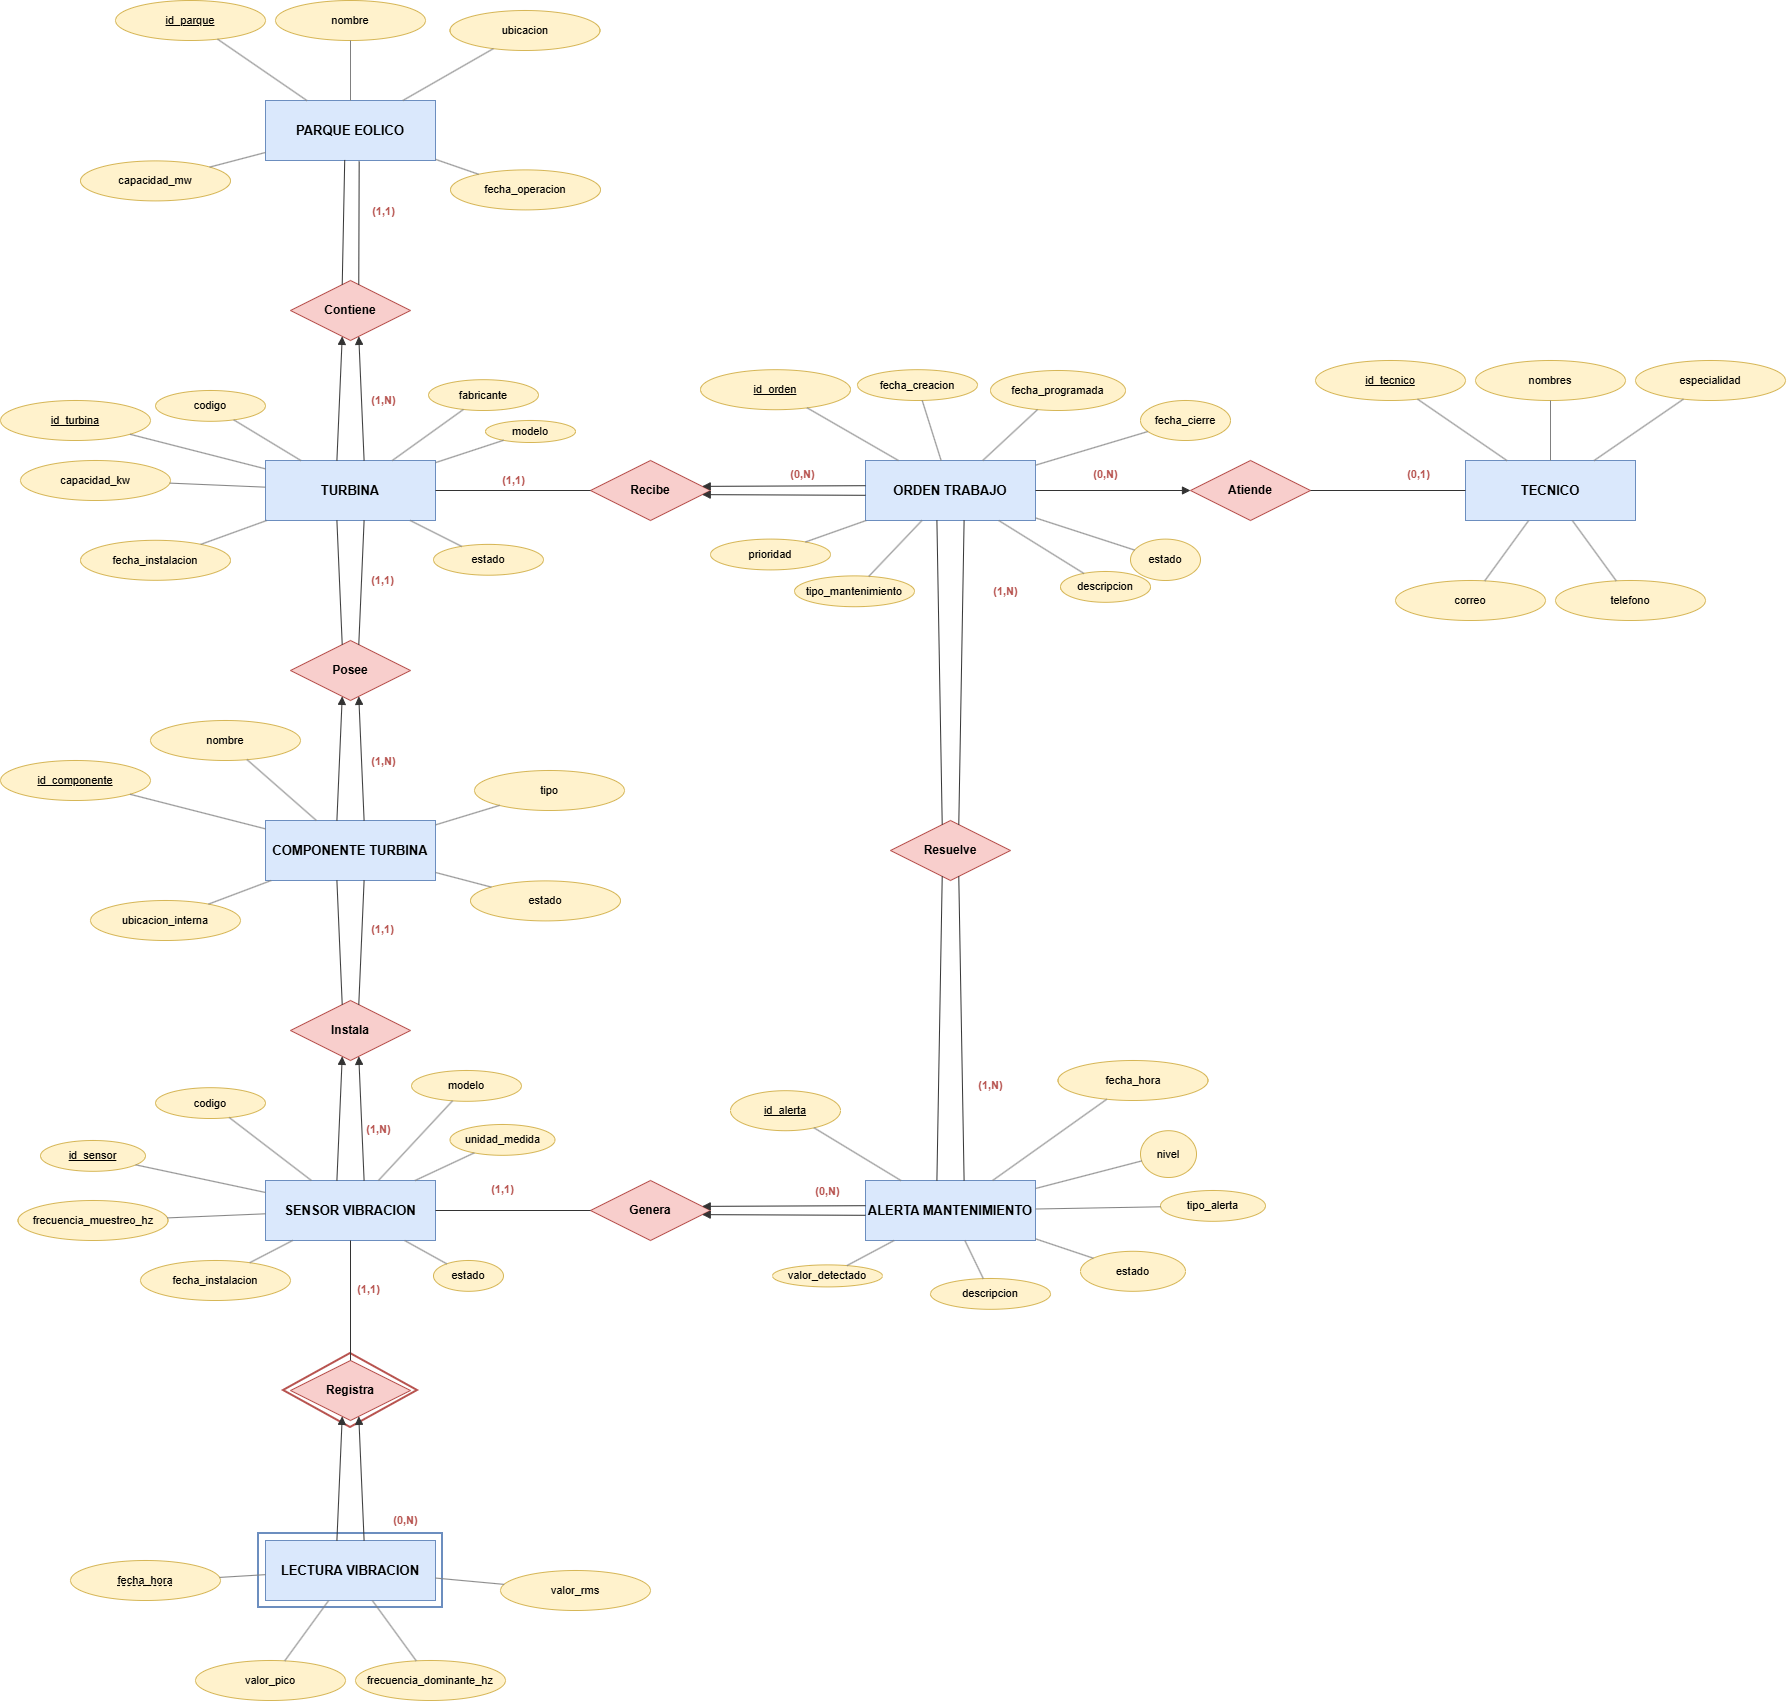
\includegraphics[width=\textwidth,height=0.8\textheight,keepaspectratio]{diagrama.png}
    \caption{Diagrama Entidad-Relación}
    \label{fig:diagrama_er}
\end{figure}

\subsection{Especificaciones y consideraciones sobre el modelo}
Debido a la cantidad de entidades y atributos, algunos detalles del diagrama de la
Figura~\ref{fig:diagrama_er} pueden resultar difíciles de leer en el documento. Por
ello, el diagrama en alta resolución se encuentra disponible en el siguiente enlace:
\begin{center}
    \href{https://drive.google.com/file/d/1enLfiX_h3VraAwfyqAF0i43-nNNw1kzT/view?usp=drive_link}{\textbf{Ver diagrama Entidad-Relación}}
\end{center}

\subsubsection{Entidad ParqueEolico}
\begin{itemize}
    \item \textbf{Especificaciones:} Almacena la información general de cada parque:
    nombre, ubicación, capacidad instalada y fecha de inicio de operación.
    \item \textbf{Consideraciones:} Es una entidad fuerte con
    \textit{id\_parque} como llave primaria.
    \item \textbf{Relaciones:} Relación 1:N con \texttt{Turbina} (\textit{Contiene}).
\end{itemize}

\subsubsection{Entidad Turbina}
\begin{itemize}
    \item \textbf{Especificaciones:} Representa cada unidad eólica y almacena código,
    fabricante, modelo, capacidad, fecha de instalación y estado.
    \item \textbf{Consideraciones:} Es una entidad fuerte identificada por
    \textit{id\_turbina}. Cada turbina pertenece obligatoriamente a un parque.
    \item \textbf{Relaciones:}
    \begin{itemize}
        \item Relación N:1 con \texttt{ParqueEolico} (\textit{Contiene}).
        \item Relación 1:N con \texttt{ComponenteTurbina} (\textit{Posee}).
        \item Relación 1:N con \texttt{OrdenTrabajo} (\textit{Recibe}).
    \end{itemize}
\end{itemize}

\subsubsection{Entidad ComponenteTurbina}
\begin{itemize}
    \item \textbf{Especificaciones:} Representa las partes internas o mecánicas que
    serán monitoreadas, como generador, caja multiplicadora o rodamiento.
    \item \textbf{Consideraciones:} Es una entidad fuerte con
    \textit{id\_componente} como llave primaria.
    \item \textbf{Relaciones:}
    \begin{itemize}
        \item Relación N:1 con \texttt{Turbina} (\textit{Posee}).
        \item Relación 1:N con \texttt{SensorVibracion} (\textit{Instala}).
    \end{itemize}
\end{itemize}

\subsubsection{Entidad SensorVibracion}
\begin{itemize}
    \item \textbf{Especificaciones:} Registra los dispositivos utilizados para medir
    vibraciones, incluyendo código, modelo, unidad, frecuencia de muestreo, fecha de
    instalación y estado.
    \item \textbf{Consideraciones:} Es una entidad fuerte con \textit{id\_sensor}
    como llave primaria. Cada sensor queda asociado a un componente específico.
    \item \textbf{Relaciones:}
    \begin{itemize}
        \item Relación N:1 con \texttt{ComponenteTurbina} (\textit{Instala}).
        \item Relación 1:N con \texttt{LecturaVibracion} (\textit{Registra}).
        \item Relación 1:N con \texttt{AlertaMantenimiento} (\textit{Genera}).
    \end{itemize}
\end{itemize}

\subsubsection{Entidad LecturaVibracion}
\begin{itemize}
    \item \textbf{Especificaciones:} Guarda las mediciones históricas de vibración:
    fecha y hora, valor RMS, valor pico y frecuencia dominante.
    \item \textbf{Consideraciones:} Se modela como una entidad débil por identidad,
    dependiente de \texttt{SensorVibracion}. Su llave primaria es compuesta por
    (\textit{id\_sensor} + \textit{fecha\_hora}), donde \textit{fecha\_hora} actúa
    como llave parcial.
    \item \textbf{Relaciones:}
    \begin{itemize}
        \item Relación N:1 con \texttt{SensorVibracion} (\textit{Registra}).
        \item Relación 1:N con \texttt{AlertaMantenimiento} (\textit{Origina}),
        con participación parcial en ambos lados.
    \end{itemize}
\end{itemize}

\subsubsection{Entidad AlertaMantenimiento}
\begin{itemize}
    \item \textbf{Especificaciones:} Registra una condición que requiere revisión,
    almacenando fecha, nivel, tipo de alerta, valor detectado, descripción y estado.
    \item \textbf{Consideraciones:} Es una entidad fuerte identificada mediante
    \textit{id\_alerta}. La referencia a la lectura de origen es opcional.
    \item \textbf{Relaciones:}
    \begin{itemize}
        \item Relación N:1 con \texttt{SensorVibracion} (\textit{Genera}).
        \item Relación N:1 con \texttt{LecturaVibracion} (\textit{Origina}).
        \item Relación N:M con \texttt{OrdenTrabajo} (\textit{Resuelve}).
    \end{itemize}
\end{itemize}

\subsubsection{Entidad Tecnico}
\begin{itemize}
    \item \textbf{Especificaciones:} Registra al personal encargado de las
    intervenciones de mantenimiento.
    \item \textbf{Consideraciones:} Entidad fuerte con \textit{id\_tecnico} como
    llave primaria.
    \item \textbf{Relaciones:} Relación 1:N con \texttt{OrdenTrabajo}
    (\textit{Atiende}).
\end{itemize}

\subsubsection{Entidad OrdenTrabajo}
\begin{itemize}
    \item \textbf{Especificaciones:} Representa una actividad de inspección,
    mantenimiento preventivo o reparación. Almacena fechas, prioridad, tipo,
    descripción y estado.
    \item \textbf{Consideraciones:} Entidad fuerte con \textit{id\_orden} como llave
    primaria. La asignación a un técnico puede ser nula mientras la orden se encuentre
    pendiente.
    \item \textbf{Relaciones:}
    \begin{itemize}
        \item Relación N:1 con \texttt{Turbina} (\textit{Recibe}).
        \item Relación N:1 con \texttt{Tecnico} (\textit{Atiende}).
        \item Relación N:M con \texttt{AlertaMantenimiento} (\textit{Resuelve}).
    \end{itemize}
\end{itemize}

% ==========================================
%          SECCIÓN 3: MODELO RELACIONAL
% ==========================================
\newpage
\section{Modelo Relacional}

\subsection{Modelo Relacional}

Las llaves primarias se indican subrayadas y las llaves foráneas con la notación
\textit{Tabla.atributo}, que señala la relación a la que hacen referencia.

\begin{itemize}

    \item \textbf{\textcolor{green!50!black}{ParqueEolico}}(
    \underline{\textcolor{blue}{id\_parque}},
    \textcolor{blue}{nombre},
    \textcolor{blue}{ubicacion},
    \textcolor{blue}{capacidad\_mw},
    \textcolor{blue}{fecha\_operacion})

    \item \textbf{\textcolor{green!50!black}{Turbina}}(
    \underline{\textcolor{blue}{id\_turbina}},
    \textcolor{blue}{ParqueEolico.id\_parque},
    \textcolor{blue}{codigo},
    \textcolor{blue}{fabricante},
    \textcolor{blue}{modelo},
    \textcolor{blue}{capacidad\_kw},
    \textcolor{blue}{fecha\_instalacion},
    \textcolor{blue}{estado})

    \item \textbf{\textcolor{green!50!black}{ComponenteTurbina}}(
    \underline{\textcolor{blue}{id\_componente}},
    \textcolor{blue}{Turbina.id\_turbina},
    \textcolor{blue}{nombre},
    \textcolor{blue}{tipo},
    \textcolor{blue}{ubicacion\_interna},
    \textcolor{blue}{estado})

    \item \textbf{\textcolor{green!50!black}{SensorVibracion}}(
    \underline{\textcolor{blue}{id\_sensor}},
    \textcolor{blue}{ComponenteTurbina.id\_componente},
    \textcolor{blue}{codigo},
    \textcolor{blue}{modelo},
    \textcolor{blue}{unidad\_medida},
    \textcolor{blue}{frecuencia\_muestreo\_hz},
    \textcolor{blue}{fecha\_instalacion},
    \textcolor{blue}{estado})

    \item \textbf{\textcolor{green!50!black}{LecturaVibracion}}(
    \underline{\textcolor{blue}{SensorVibracion.id\_sensor}},
    \underline{\textcolor{blue}{fecha\_hora}},
    \textcolor{blue}{valor\_rms},
    \textcolor{blue}{valor\_pico},
    \textcolor{blue}{frecuencia\_dominante\_hz})

    \item \textbf{\textcolor{green!50!black}{AlertaMantenimiento}}(
    \underline{\textcolor{blue}{id\_alerta}},
    \textcolor{blue}{SensorVibracion.id\_sensor},
    \textcolor{blue}{LecturaVibracion.fecha\_hora\_lectura},
    \textcolor{blue}{fecha\_hora},
    \textcolor{blue}{nivel},
    \textcolor{blue}{tipo\_alerta},
    \textcolor{blue}{valor\_detectado},
    \textcolor{blue}{descripcion},
    \textcolor{blue}{estado})

    \item \textbf{\textcolor{green!50!black}{Tecnico}}(
    \underline{\textcolor{blue}{id\_tecnico}},
    \textcolor{blue}{nombres},
    \textcolor{blue}{especialidad},
    \textcolor{blue}{correo},
    \textcolor{blue}{telefono})

    \item \textbf{\textcolor{green!50!black}{OrdenTrabajo}}(
    \underline{\textcolor{blue}{id\_orden}},
    \textcolor{blue}{Turbina.id\_turbina},
    \textcolor{blue}{Tecnico.id\_tecnico},
    \textcolor{blue}{fecha\_creacion},
    \textcolor{blue}{fecha\_programada},
    \textcolor{blue}{fecha\_cierre},
    \textcolor{blue}{prioridad},
    \textcolor{blue}{tipo\_mantenimiento},
    \textcolor{blue}{descripcion},
    \textcolor{blue}{estado})

    \item \textbf{\textcolor{green!50!black}{AlertaOrden}}(
    \underline{\textcolor{blue}{AlertaMantenimiento.id\_alerta}},
    \underline{\textcolor{blue}{OrdenTrabajo.id\_orden}})

\end{itemize}

En \texttt{AlertaMantenimiento}, el par (\textit{id\_sensor},
\textit{fecha\_hora\_lectura}) forma una llave foránea compuesta hacia
\texttt{LecturaVibracion}. Al reutilizar \textit{id\_sensor}, se garantiza que la
lectura de origen pertenezca al mismo sensor que generó la alerta.

\subsubsection{Restricciones de integridad}

Además de las llaves primarias y foráneas indicadas, el modelo contempla las
siguientes restricciones:

\begin{itemize}
    \item \textbf{Unicidad (UNIQUE):} \textit{Turbina.codigo},
    \textit{SensorVibracion.codigo} y \textit{Tecnico.correo} no pueden repetirse.

    \item \textbf{Dominios (CHECK):}
    \begin{itemize}
        \item \textit{Turbina.estado} $\in$ \{Operativa, Detenida, Mantenimiento\}.
        \item \textit{SensorVibracion.estado} $\in$ \{Activo, Inactivo, Mantenimiento\}.
        \item \textit{AlertaMantenimiento.nivel} y \textit{OrdenTrabajo.prioridad}
        $\in$ \{Baja, Media, Alta, Critica\}.
        \item \textit{AlertaMantenimiento.estado} $\in$ \{Abierta, En revision, Cerrada\}.
        \item \textit{OrdenTrabajo.tipo\_mantenimiento} $\in$ \{Inspeccion, Preventivo,
        Correctivo\}.
        \item \textit{OrdenTrabajo.estado} $\in$ \{Pendiente, En proceso, Finalizada,
        Cancelada\}.
    \end{itemize}

    \item \textbf{Valores numéricos (CHECK):} \textit{valor\_rms},
    \textit{valor\_pico} y \textit{frecuencia\_dominante\_hz} deben ser $\geq 0$;
    \textit{capacidad\_mw}, \textit{capacidad\_kw} y
    \textit{frecuencia\_muestreo\_hz} deben ser $> 0$.

    \item \textbf{Fechas (CHECK):} \textit{fecha\_cierre} es nula o mayor o igual que
    \textit{fecha\_creacion} en \texttt{OrdenTrabajo}.

    \item \textbf{Estado de la orden (CHECK):} una orden en estado En proceso o
    Finalizada debe tener \textit{id\_tecnico} no nulo, y una orden Finalizada debe
    tener \textit{fecha\_cierre} registrada.

    \item \textbf{Consistencia entre tablas (trigger en el Hito 2):} al insertar en
    \texttt{AlertaOrden}, la turbina a la que pertenece el sensor de la alerta
    (sensor $\rightarrow$ componente $\rightarrow$ turbina) debe coincidir con
    \textit{OrdenTrabajo.id\_turbina}.
\end{itemize}

\subsubsection{Normalización}

El modelo se encuentra en Forma Normal de Boyce-Codd (FNBC):

\begin{itemize}
    \item \textbf{1FN:} Todos los atributos son atómicos y no existen grupos
    repetitivos. Por ejemplo, cada lectura se almacena como una fila independiente en
    lugar de guardar varias mediciones en un mismo registro del sensor.

    \item \textbf{2FN:} Las únicas tablas con llave compuesta son
    \texttt{LecturaVibracion} y \texttt{AlertaOrden}. En la primera, los valores
    medidos dependen del sensor \textit{y} del instante de medición, no de solo una
    parte de la llave; la segunda no tiene atributos fuera de la llave.

    \item \textbf{3FN y FNBC:} No existen dependencias transitivas. Por ejemplo,
    \texttt{OrdenTrabajo} no almacena el parque ni el nombre del técnico, ya que se
    obtienen a través de \textit{id\_turbina} e \textit{id\_tecnico}. Los únicos
    determinantes de cada tabla son su llave primaria y las llaves candidatas
    declaradas como únicas (\textit{codigo} en \texttt{Turbina} y
    \texttt{SensorVibracion}, \textit{correo} en \texttt{Tecnico}).
\end{itemize}

\subsection{Especificaciones de transformación}

\subsubsection{Entidades}

Para transformar las entidades fuertes del sistema se aplicaron las siguientes
especificaciones:

\begin{itemize}
    \item \textbf{ParqueEolico}: Se crea una relación con
    \textit{id\_parque} como llave primaria.

    \item \textbf{Turbina}: Se crea una relación con
    \textit{id\_turbina} como llave primaria. Recibe \textit{id\_parque} como llave
    foránea debido a la relación 1:N con \texttt{ParqueEolico}.

    \item \textbf{ComponenteTurbina}: Se crea con \textit{id\_componente} como PK y
    recibe \textit{id\_turbina} como FK.

    \item \textbf{SensorVibracion}: Se crea con \textit{id\_sensor} como PK y recibe
    \textit{id\_componente} como FK.

    \item \textbf{AlertaMantenimiento}: Se crea con \textit{id\_alerta} como PK.
    Recibe \textit{id\_sensor} como FK hacia \texttt{SensorVibracion} y el par
    (\textit{id\_sensor}, \textit{fecha\_hora\_lectura}) como FK compuesta opcional
    hacia \texttt{LecturaVibracion}.

    \item \textbf{Tecnico}: Se crea con \textit{id\_tecnico} como PK.

    \item \textbf{OrdenTrabajo}: Se crea con \textit{id\_orden} como PK. Recibe
    \textit{id\_turbina} e \textit{id\_tecnico} como llaves foráneas.
\end{itemize}

\subsubsection{Entidades débiles}

\begin{itemize}
    \item \textbf{LecturaVibracion}: Se considera una entidad débil por identidad
    vinculada a \texttt{SensorVibracion}, ya que una lectura no tiene sentido sin el
    sensor que la produjo. Su llave primaria se compone de
    \textit{id\_sensor} y \textit{fecha\_hora}. El atributo
    \textit{id\_sensor} es simultáneamente PK parcial y FK.
\end{itemize}

\subsubsection{Entidades superclase/subclases}

El modelo no utiliza relaciones de generalización o especialización. Ninguna entidad
fue dividida en superclases o subclases porque los objetos principales poseen
atributos y comportamientos suficientemente distintos para modelarse de manera
independiente.

\subsubsection{Relaciones binarias}

\textbf{Relaciones binarias no modeladas como tablas independientes:}

\begin{itemize}
    \item \textbf{Contiene}: Relaciona \texttt{ParqueEolico} con \texttt{Turbina}.
    Un parque puede contener muchas turbinas y cada turbina pertenece a un solo
    parque. La llave \textit{id\_parque} se propaga hacia \texttt{Turbina}.

    \item \textbf{Posee}: Relaciona \texttt{Turbina} con
    \texttt{ComponenteTurbina}. La llave \textit{id\_turbina} se propaga hacia
    \texttt{ComponenteTurbina}.

    \item \textbf{Instala}: Relaciona \texttt{ComponenteTurbina} con
    \texttt{SensorVibracion}. La llave \textit{id\_componente} se propaga hacia
    \texttt{SensorVibracion}.

    \item \textbf{Registra}: Relaciona \texttt{SensorVibracion} con
    \texttt{LecturaVibracion}. El identificador del sensor forma parte de la llave
    compuesta de la entidad débil.

    \item \textbf{Genera}: Relaciona \texttt{SensorVibracion} con
    \texttt{AlertaMantenimiento}. La llave \textit{id\_sensor} se propaga hacia la
    alerta.

    \item \textbf{Origina}: Relaciona \texttt{LecturaVibracion} con
    \texttt{AlertaMantenimiento}. La llave compuesta de la lectura se propaga hacia la
    alerta reutilizando \textit{id\_sensor} y agregando \textit{fecha\_hora\_lectura},
    que puede ser nula.

    \item \textbf{Recibe}: Relaciona \texttt{Turbina} con \texttt{OrdenTrabajo}.
    La llave \textit{id\_turbina} se propaga hacia la orden.

    \item \textbf{Atiende}: Relaciona \texttt{Tecnico} con \texttt{OrdenTrabajo}.
    La llave \textit{id\_tecnico} se incorpora en \texttt{OrdenTrabajo}. Puede ser
    nula mientras la orden no haya sido asignada.
\end{itemize}

\textbf{Relaciones binarias modeladas:}

\begin{itemize}
    \item \textbf{Resuelve}: La relación entre \texttt{AlertaMantenimiento} y
    \texttt{OrdenTrabajo} es muchos a muchos (N:M). Por ello se crea la tabla
    \texttt{AlertaOrden}, cuya llave primaria está formada por
    (\textit{id\_alerta}, \textit{id\_orden}); ambos atributos son también llaves
    foráneas.
\end{itemize}

\subsubsection{Relaciones ternarias}

El modelo propuesto no contiene relaciones ternarias. Las reglas del dominio pueden
representarse correctamente mediante relaciones binarias y una relación asociativa
N:M entre alertas y órdenes.

% ==========================================
%       SECCIÓN 3.3: DICCIONARIO DE DATOS
% ==========================================
\subsection{Diccionario de datos}

En la columna \textbf{Clave}, PK indica llave primaria, FK llave foránea y UK
restricción de unicidad.

\par\bigskip

% 1. PARQUE EOLICO
\subsubsection{Tabla: ParqueEolico}
\begin{table}[H]
\centering
\small
\caption{Diccionario de datos de la tabla \texttt{ParqueEolico}}
\begin{tabular}{|l|l|c|c|c|p{5.1cm}|}
\hline
\textbf{Campo} & \textbf{Tipo de Dato} & \textbf{Long.} & \textbf{Clave} & \textbf{Nulo} & \textbf{Descripción} \\ \hline
\texttt{id\_parque} & INT & - & PK & NO & Identificador único del parque eólico. \\ \hline
\texttt{nombre} & VARCHAR & 100 & - & NO & Nombre utilizado para identificar el parque. \\ \hline
\texttt{ubicacion} & VARCHAR & 150 & - & NO & Ubicación general del parque eólico. \\ \hline
\texttt{capacidad\_mw} & DECIMAL & 10,2 & - & NO & Capacidad instalada del parque en MW. \\ \hline
\texttt{fecha\_operacion} & DATE & - & - & NO & Fecha de inicio de operación registrada. \\ \hline
\end{tabular}
\end{table}

% 2. TURBINA
\subsubsection{Tabla: Turbina}
\begin{table}[H]
\centering
\small
\caption{Diccionario de datos de la tabla \texttt{Turbina}}
\begin{tabular}{|l|l|c|c|c|p{5.1cm}|}
\hline
\textbf{Campo} & \textbf{Tipo de Dato} & \textbf{Long.} & \textbf{Clave} & \textbf{Nulo} & \textbf{Descripción} \\ \hline
\texttt{id\_turbina} & INT & - & PK & NO & Identificador único de la turbina. \\ \hline
\texttt{id\_parque} & INT & - & FK & NO & Parque eólico al que pertenece. \\ \hline
\texttt{codigo} & VARCHAR & 30 & UK & NO & Código interno único de la turbina. \\ \hline
\texttt{fabricante} & VARCHAR & 60 & - & NO & Fabricante del equipo. \\ \hline
\texttt{modelo} & VARCHAR & 60 & - & NO & Modelo de la turbina. \\ \hline
\texttt{capacidad\_kw} & DECIMAL & 10,2 & - & NO & Potencia nominal en kW. \\ \hline
\texttt{fecha\_instalacion} & DATE & - & - & NO & Fecha de instalación de la turbina. \\ \hline
\texttt{estado} & VARCHAR & 20 & - & NO & Estado: Operativa, Detenida o Mantenimiento. \\ \hline
\end{tabular}
\end{table}

% 3. COMPONENTE
\subsubsection{Tabla: ComponenteTurbina}
\begin{table}[H]
\centering
\small
\caption{Diccionario de datos de la tabla \texttt{ComponenteTurbina}}
\begin{tabular}{|l|l|c|c|c|p{5.1cm}|}
\hline
\textbf{Campo} & \textbf{Tipo de Dato} & \textbf{Long.} & \textbf{Clave} & \textbf{Nulo} & \textbf{Descripción} \\ \hline
\texttt{id\_componente} & INT & - & PK & NO & Identificador único del componente. \\ \hline
\texttt{id\_turbina} & INT & - & FK & NO & Turbina a la que pertenece. \\ \hline
\texttt{nombre} & VARCHAR & 60 & - & NO & Nombre del componente monitoreado. \\ \hline
\texttt{tipo} & VARCHAR & 40 & - & NO & Clasificación del componente. \\ \hline
\texttt{ubicacion\_interna} & VARCHAR & 60 & - & NO & Ubicación del componente dentro de la turbina. \\ \hline
\texttt{estado} & VARCHAR & 20 & - & NO & Estado operativo del componente. \\ \hline
\end{tabular}
\end{table}

% 4. SENSOR
\subsubsection{Tabla: SensorVibracion}
\begin{table}[H]
\centering
\small
\caption{Diccionario de datos de la tabla \texttt{SensorVibracion}}
\begin{tabular}{|l|l|c|c|c|p{5.1cm}|}
\hline
\textbf{Campo} & \textbf{Tipo de Dato} & \textbf{Long.} & \textbf{Clave} & \textbf{Nulo} & \textbf{Descripción} \\ \hline
\texttt{id\_sensor} & INT & - & PK & NO & Identificador único del sensor. \\ \hline
\texttt{id\_componente} & INT & - & FK & NO & Componente en el que se encuentra instalado. \\ \hline
\texttt{codigo} & VARCHAR & 30 & UK & NO & Código interno único del sensor. \\ \hline
\texttt{modelo} & VARCHAR & 50 & - & NO & Modelo o referencia del dispositivo. \\ \hline
\texttt{unidad\_medida} & VARCHAR & 20 & - & NO & Unidad utilizada para registrar vibración. \\ \hline
\texttt{frecuencia\_muestreo\_hz} & DECIMAL & 10,2 & - & NO & Frecuencia de muestreo configurada. \\ \hline
\texttt{fecha\_instalacion} & DATE & - & - & NO & Fecha de instalación del sensor. \\ \hline
\texttt{estado} & VARCHAR & 20 & - & NO & Estado: Activo, Inactivo o Mantenimiento. \\ \hline
\end{tabular}
\end{table}

% 5. LECTURA
\subsubsection{Tabla: LecturaVibracion}
\begin{table}[H]
\centering
\small
\caption{Diccionario de datos de la tabla \texttt{LecturaVibracion}}
\begin{tabular}{|l|l|c|c|c|p{5.1cm}|}
\hline
\textbf{Campo} & \textbf{Tipo de Dato} & \textbf{Long.} & \textbf{Clave} & \textbf{Nulo} & \textbf{Descripción} \\ \hline
\texttt{id\_sensor} & INT & - & PK, FK & NO & Sensor que produjo la lectura. \\ \hline
\texttt{fecha\_hora} & TIMESTAMP & - & PK & NO & Momento exacto de la medición. \\ \hline
\texttt{valor\_rms} & DECIMAL & 12,4 & - & NO & Valor RMS de vibración registrado. \\ \hline
\texttt{valor\_pico} & DECIMAL & 12,4 & - & NO & Valor pico registrado durante la medición. \\ \hline
\texttt{frecuencia\_dominante\_hz} & DECIMAL & 12,4 & - & NO & Frecuencia dominante observada en Hz. \\ \hline
\end{tabular}
\end{table}

% 6. ALERTA
\subsubsection{Tabla: AlertaMantenimiento}
\begin{table}[H]
\centering
\small
\caption{Diccionario de datos de la tabla \texttt{AlertaMantenimiento}}
\begin{tabular}{|l|l|c|c|c|p{5.1cm}|}
\hline
\textbf{Campo} & \textbf{Tipo de Dato} & \textbf{Long.} & \textbf{Clave} & \textbf{Nulo} & \textbf{Descripción} \\ \hline
\texttt{id\_alerta} & BIGINT & - & PK & NO & Identificador único de la alerta. \\ \hline
\texttt{id\_sensor} & INT & - & FK & NO & Sensor que originó la alerta. \\ \hline
\texttt{fecha\_hora\_lectura} & TIMESTAMP & - & FK & SÍ & Junto con \texttt{id\_sensor}, referencia la lectura que originó la alerta; nulo si la alerta fue registrada manualmente. \\ \hline
\texttt{fecha\_hora} & TIMESTAMP & - & - & NO & Momento de generación de la alerta. \\ \hline
\texttt{nivel} & VARCHAR & 15 & - & NO & Prioridad: Baja, Media, Alta o Critica. \\ \hline
\texttt{tipo\_alerta} & VARCHAR & 50 & - & NO & Clasificación de la condición detectada. \\ \hline
\texttt{valor\_detectado} & DECIMAL & 12,4 & - & NO & Valor relacionado con la condición anormal. \\ \hline
\texttt{descripcion} & VARCHAR & 255 & - & NO & Descripción de la alerta generada. \\ \hline
\texttt{estado} & VARCHAR & 20 & - & NO & Abierta, En revision o Cerrada. \\ \hline
\end{tabular}
\end{table}

% 7. TECNICO
\subsubsection{Tabla: Tecnico}
\begin{table}[H]
\centering
\small
\caption{Diccionario de datos de la tabla \texttt{Tecnico}}
\begin{tabular}{|l|l|c|c|c|p{5.1cm}|}
\hline
\textbf{Campo} & \textbf{Tipo de Dato} & \textbf{Long.} & \textbf{Clave} & \textbf{Nulo} & \textbf{Descripción} \\ \hline
\texttt{id\_tecnico} & INT & - & PK & NO & Identificador único del técnico. \\ \hline
\texttt{nombres} & VARCHAR & 100 & - & NO & Nombres y apellidos del responsable. \\ \hline
\texttt{especialidad} & VARCHAR & 60 & - & NO & Área técnica principal del trabajador. \\ \hline
\texttt{correo} & VARCHAR & 100 & UK & NO & Correo de contacto. \\ \hline
\texttt{telefono} & VARCHAR & 15 & - & SÍ & Teléfono de contacto. \\ \hline
\end{tabular}
\end{table}

% 8. ORDEN
\subsubsection{Tabla: OrdenTrabajo}
\begin{table}[H]
\centering
\small
\caption{Diccionario de datos de la tabla \texttt{OrdenTrabajo}}
\begin{tabular}{|l|l|c|c|c|p{5.1cm}|}
\hline
\textbf{Campo} & \textbf{Tipo de Dato} & \textbf{Long.} & \textbf{Clave} & \textbf{Nulo} & \textbf{Descripción} \\ \hline
\texttt{id\_orden} & BIGINT & - & PK & NO & Identificador único de la orden. \\ \hline
\texttt{id\_turbina} & INT & - & FK & NO & Turbina sobre la que se realizará el trabajo. \\ \hline
\texttt{id\_tecnico} & INT & - & FK & SÍ & Técnico responsable; puede ser nulo antes de asignarse. \\ \hline
\texttt{fecha\_creacion} & TIMESTAMP & - & - & NO & Fecha y hora de creación de la orden. \\ \hline
\texttt{fecha\_programada} & TIMESTAMP & - & - & SÍ & Fecha prevista para la intervención. \\ \hline
\texttt{fecha\_cierre} & TIMESTAMP & - & - & SÍ & Fecha de finalización de la orden. \\ \hline
\texttt{prioridad} & VARCHAR & 15 & - & NO & Baja, Media, Alta o Critica. \\ \hline
\texttt{tipo\_mantenimiento} & VARCHAR & 50 & - & NO & Inspeccion, Preventivo o Correctivo. \\ \hline
\texttt{descripcion} & VARCHAR & 255 & - & NO & Descripción del trabajo requerido. \\ \hline
\texttt{estado} & VARCHAR & 20 & - & NO & Pendiente, En proceso, Finalizada o Cancelada. \\ \hline
\end{tabular}
\end{table}

% 9. ALERTA ORDEN
\subsubsection{Tabla: AlertaOrden}
\begin{table}[H]
\centering
\small
\caption{Diccionario de datos de la tabla \texttt{AlertaOrden}}
\begin{tabular}{|l|l|c|c|c|p{5.1cm}|}
\hline
\textbf{Campo} & \textbf{Tipo de Dato} & \textbf{Long.} & \textbf{Clave} & \textbf{Nulo} & \textbf{Descripción} \\ \hline
\texttt{id\_alerta} & BIGINT & - & PK, FK & NO & Alerta atendida o relacionada con la orden. \\ \hline
\texttt{id\_orden} & BIGINT & - & PK, FK & NO & Orden de trabajo vinculada a la alerta. \\ \hline
\end{tabular}
\end{table}

\newpage
\section{Implementación de la base de datos}

\subsection{Creación de Tablas en PostgreSQL}

Se implementó el modelo relacional del Hito 1 en PostgreSQL. Las decisiones
principales fueron: (i) claves sustitutas con
\texttt{GENERATED BY DEFAULT AS IDENTITY}, (ii) todas las reglas de dominio del
Hito 1 como restricciones \texttt{CHECK}, y (iii) la clave foránea compuesta
\texttt{(id\_sensor, fecha\_hora\_lectura)} de \texttt{AlertaMantenimiento}
hacia \texttt{LecturaVibracion}, que con \texttt{MATCH SIMPLE} permite que la
lectura sea nula en alertas manuales.

\begin{lstlisting}
CREATE TABLE ParqueEolico (
  id_parque        INT GENERATED BY DEFAULT AS IDENTITY PRIMARY KEY,
  nombre           VARCHAR(100) NOT NULL,
  ubicacion        VARCHAR(150) NOT NULL,
  capacidad_mw     DECIMAL(10,2) NOT NULL CHECK (capacidad_mw > 0),
  fecha_operacion  DATE NOT NULL
);

CREATE TABLE Turbina (
  id_turbina        INT GENERATED BY DEFAULT AS IDENTITY PRIMARY KEY,
  id_parque         INT NOT NULL REFERENCES ParqueEolico(id_parque),
  codigo            VARCHAR(30) NOT NULL UNIQUE,
  fabricante        VARCHAR(60) NOT NULL,
  modelo            VARCHAR(60) NOT NULL,
  capacidad_kw      DECIMAL(10,2) NOT NULL CHECK (capacidad_kw > 0),
  fecha_instalacion DATE NOT NULL,
  estado            VARCHAR(20) NOT NULL
    CHECK (estado IN ('Operativa','Detenida','Mantenimiento'))
);

CREATE TABLE ComponenteTurbina (
  id_componente     INT GENERATED BY DEFAULT AS IDENTITY PRIMARY KEY,
  id_turbina        INT NOT NULL REFERENCES Turbina(id_turbina),
  nombre            VARCHAR(60) NOT NULL,
  tipo              VARCHAR(40) NOT NULL,
  ubicacion_interna VARCHAR(60) NOT NULL,
  estado            VARCHAR(20) NOT NULL
);

CREATE TABLE SensorVibracion (
  id_sensor             INT GENERATED BY DEFAULT AS IDENTITY PRIMARY KEY,
  id_componente         INT NOT NULL REFERENCES ComponenteTurbina(id_componente),
  codigo                VARCHAR(30) NOT NULL UNIQUE,
  modelo                VARCHAR(50) NOT NULL,
  unidad_medida         VARCHAR(20) NOT NULL,
  frecuencia_muestreo_hz DECIMAL(10,2) NOT NULL CHECK (frecuencia_muestreo_hz > 0),
  fecha_instalacion     DATE NOT NULL,
  estado                VARCHAR(20) NOT NULL
    CHECK (estado IN ('Activo','Inactivo','Mantenimiento'))
);

CREATE TABLE LecturaVibracion (
  id_sensor   INT NOT NULL REFERENCES SensorVibracion(id_sensor),
  fecha_hora  TIMESTAMP NOT NULL,
  valor_rms   DECIMAL(12,4) NOT NULL CHECK (valor_rms >= 0),
  valor_pico  DECIMAL(12,4) NOT NULL CHECK (valor_pico >= 0),
  frecuencia_dominante_hz DECIMAL(12,4) NOT NULL CHECK (frecuencia_dominante_hz >= 0),
  PRIMARY KEY (id_sensor, fecha_hora)
);

CREATE TABLE Tecnico (
  id_tecnico   INT GENERATED BY DEFAULT AS IDENTITY PRIMARY KEY,
  nombres      VARCHAR(100) NOT NULL,
  especialidad VARCHAR(60) NOT NULL,
  correo       VARCHAR(100) NOT NULL UNIQUE,
  telefono     VARCHAR(15)
);

CREATE TABLE AlertaMantenimiento (
  id_alerta          BIGINT GENERATED BY DEFAULT AS IDENTITY PRIMARY KEY,
  id_sensor          INT NOT NULL REFERENCES SensorVibracion(id_sensor),
  fecha_hora_lectura TIMESTAMP,
  fecha_hora         TIMESTAMP NOT NULL,
  nivel              VARCHAR(15) NOT NULL
    CHECK (nivel IN ('Baja','Media','Alta','Critica')),
  tipo_alerta        VARCHAR(50) NOT NULL,
  valor_detectado    DECIMAL(12,4) NOT NULL,
  descripcion        VARCHAR(255) NOT NULL,
  estado             VARCHAR(20) NOT NULL
    CHECK (estado IN ('Abierta','En revision','Cerrada')),
  FOREIGN KEY (id_sensor, fecha_hora_lectura)
    REFERENCES LecturaVibracion(id_sensor, fecha_hora)
);

CREATE TABLE OrdenTrabajo (
  id_orden           BIGINT GENERATED BY DEFAULT AS IDENTITY PRIMARY KEY,
  id_turbina         INT NOT NULL REFERENCES Turbina(id_turbina),
  id_tecnico         INT REFERENCES Tecnico(id_tecnico),
  fecha_creacion     TIMESTAMP NOT NULL,
  fecha_programada   TIMESTAMP,
  fecha_cierre       TIMESTAMP,
  prioridad          VARCHAR(15) NOT NULL
    CHECK (prioridad IN ('Baja','Media','Alta','Critica')),
  tipo_mantenimiento VARCHAR(50) NOT NULL
    CHECK (tipo_mantenimiento IN ('Inspeccion','Preventivo','Correctivo')),
  descripcion        VARCHAR(255) NOT NULL,
  estado             VARCHAR(20) NOT NULL
    CHECK (estado IN ('Pendiente','En proceso','Finalizada','Cancelada')),
  CHECK (fecha_cierre IS NULL OR fecha_cierre >= fecha_creacion),
  CHECK (estado NOT IN ('En proceso','Finalizada') OR id_tecnico IS NOT NULL),
  CHECK (estado <> 'Finalizada' OR fecha_cierre IS NOT NULL)
);

CREATE TABLE AlertaOrden (
  id_alerta BIGINT NOT NULL REFERENCES AlertaMantenimiento(id_alerta),
  id_orden  BIGINT NOT NULL REFERENCES OrdenTrabajo(id_orden),
  PRIMARY KEY (id_alerta, id_orden)
);
\end{lstlisting}

\subsection{Carga de datos}

Para poblar la base de datos se desarrolló un script en SQL que genera datos
sintéticos con las funciones \texttt{generate\_series} y \texttt{random} de
PostgreSQL. Se crearon cuatro bases de datos, una por escenario de carga:
1\,000, 10\,000, 100\,000 y 1\,000\,000 de lecturas de vibración. Las tablas
maestras tienen el mismo tamaño en los cuatro escenarios (5 parques, 100
turbinas, 400 componentes, 800 sensores y 30 técnicos), mientras que las
lecturas se reparten entre los 800 sensores, una por hora, de modo que la llave
(\textit{id\_sensor}, \textit{fecha\_hora}) no se repite.

Los rangos de vibración (RMS entre 0,5 y 3 para lecturas normales y entre 4 y 6
para lecturas anómalas) se definieron como valores de referencia para la
experimentación; el conjunto de datos de Fraunhofer LBF~\cite{fraunhofer} se
tomó como referencia para la estructura de las mediciones. Cerca del 0,5\,\% de
las lecturas son anómalas y cada una genera una alerta por regla de umbral. Las
órdenes de trabajo se generan en proporción al número de lecturas y las órdenes
correctivas se vinculan con alertas de su misma turbina. El script completo se
encuentra en el repositorio indicado en los Anexos.

Como referencia, el Cuadro~\ref{tab:filas_dump} resume el número de filas de cada
tabla en las cuatro escalas. Los conteos de las tablas derivadas (alertas,
órdenes y la relación alerta--orden) dependen de la carga y varían ligeramente
cada vez que se regeneran las bases; para el informe se usaron los dumps de
\texttt{dumps/}.

\begin{table}[H]
\centering
\small
\caption{Número de filas por tabla y por escala}
\label{tab:filas_dump}
\begin{tabular}{|l|r|r|r|r|}
\hline
\textbf{Tabla} & \textbf{1k} & \textbf{10k} & \textbf{100k} & \textbf{1M} \\ \hline
ParqueEolico & 5 & 5 & 5 & 5 \\ \hline
Turbina & 100 & 100 & 100 & 100 \\ \hline
ComponenteTurbina & 400 & 400 & 400 & 400 \\ \hline
SensorVibracion & 800 & 800 & 800 & 800 \\ \hline
Tecnico & 30 & 30 & 30 & 30 \\ \hline
LecturaVibracion & 1\,000 & 10\,000 & 100\,000 & 991\,610 \\ \hline
AlertaMantenimiento & 5 & 54 & 519 & 5\,019 \\ \hline
OrdenTrabajo & 10 & 20 & 200 & 2\,000 \\ \hline
AlertaOrden & 0 & 4 & 122 & 1\,260 \\ \hline
\end{tabular}
\end{table}

\subsection{Simulación de Datos Faltantes}

El esquema contempla valores nulos en los siguientes campos:

\begin{itemize}
    \item \texttt{AlertaMantenimiento.fecha\_hora\_lectura}: es nulo cuando la
    alerta fue registrada manualmente por el analista y no proviene de una
    lectura.
    \item \texttt{OrdenTrabajo.id\_tecnico}: es nulo mientras la orden está
    pendiente y aún no fue asignada.
    \item \texttt{OrdenTrabajo.fecha\_cierre}: es nulo hasta que la orden
    finaliza.
    \item \texttt{Tecnico.telefono}: es opcional.
\end{itemize}

Además, sobre los datos cargados se simularon alertas manuales, sensores fuera
de servicio y un periodo sin lecturas:

\begin{lstlisting}
-- 2% de alertas registradas manualmente (sin lectura de origen)
UPDATE AlertaMantenimiento SET fecha_hora_lectura = NULL
WHERE random() < 0.02;

-- 5% de sensores fuera de servicio
UPDATE SensorVibracion SET estado = 'Inactivo' WHERE random() < 0.05;

-- Periodo sin lecturas en los sensores inactivos
DELETE FROM LecturaVibracion l
USING SensorVibracion s
WHERE s.id_sensor = l.id_sensor AND s.estado = 'Inactivo'
  AND l.fecha_hora BETWEEN '2026-01-10' AND '2026-01-20'
  AND NOT EXISTS (SELECT 1 FROM AlertaMantenimiento a
                  WHERE a.id_sensor = l.id_sensor
                    AND a.fecha_hora_lectura = l.fecha_hora);
\end{lstlisting}

\subsection{Views}

Se crearon tres vistas, una para cada tipo de usuario principal del sistema.

\begin{lstlisting}
-- Supervisor: turbinas con alertas Alta/Critica no cerradas
CREATE VIEW v_alertas_criticas_abiertas AS
SELECT p.nombre AS parque, t.id_turbina, t.codigo AS turbina,
       COUNT(*) AS alertas_abiertas, MAX(a.fecha_hora) AS ultima_alerta
FROM AlertaMantenimiento a
JOIN SensorVibracion s    ON s.id_sensor = a.id_sensor
JOIN ComponenteTurbina c  ON c.id_componente = s.id_componente
JOIN Turbina t            ON t.id_turbina = c.id_turbina
JOIN ParqueEolico p       ON p.id_parque = t.id_parque
WHERE a.nivel IN ('Alta','Critica') AND a.estado <> 'Cerrada'
GROUP BY p.nombre, t.id_turbina, t.codigo;

-- Analista: estadisticas mensuales de vibracion por sensor
CREATE VIEW v_estadisticas_sensor_mes AS
SELECT s.id_sensor, s.codigo, date_trunc('month', l.fecha_hora) AS mes,
       AVG(l.valor_rms) AS rms_promedio, MAX(l.valor_rms) AS rms_maximo,
       MAX(l.valor_pico) AS pico_maximo, COUNT(*) AS n_lecturas
FROM LecturaVibracion l
JOIN SensorVibracion s ON s.id_sensor = l.id_sensor
GROUP BY s.id_sensor, s.codigo, date_trunc('month', l.fecha_hora);

-- Supervisor: carga de trabajo por tecnico
CREATE VIEW v_carga_tecnico AS
SELECT tc.id_tecnico, tc.nombres, tc.especialidad,
       COUNT(*) FILTER (WHERE o.estado = 'Pendiente')  AS pendientes,
       COUNT(*) FILTER (WHERE o.estado = 'En proceso') AS en_proceso
FROM Tecnico tc
LEFT JOIN OrdenTrabajo o ON o.id_tecnico = tc.id_tecnico
GROUP BY tc.id_tecnico, tc.nombres, tc.especialidad;
\end{lstlisting}

\subsection{Procedimientos Almacenados}

Se implementaron dos procedimientos que automatizan el flujo de mantenimiento
(crear una orden a partir de una alerta y cerrar una orden) y una función que
devuelve el historial de una turbina.

\begin{lstlisting}
-- Crea una orden a partir de una alerta y la vincula
CREATE OR REPLACE PROCEDURE sp_crear_orden_desde_alerta(
    p_id_alerta BIGINT, p_id_tecnico INT, p_tipo VARCHAR, INOUT p_id_orden BIGINT)
LANGUAGE plpgsql AS $$
DECLARE v_turbina INT; v_nivel VARCHAR;
BEGIN
  SELECT c.id_turbina, a.nivel INTO v_turbina, v_nivel
  FROM AlertaMantenimiento a
  JOIN SensorVibracion s   ON s.id_sensor = a.id_sensor
  JOIN ComponenteTurbina c ON c.id_componente = s.id_componente
  WHERE a.id_alerta = p_id_alerta;

  IF v_turbina IS NULL THEN
    RAISE EXCEPTION 'La alerta % no existe', p_id_alerta;
  END IF;

  INSERT INTO OrdenTrabajo(id_turbina, id_tecnico, fecha_creacion, fecha_programada,
                           prioridad, tipo_mantenimiento, descripcion, estado)
  VALUES (v_turbina, p_id_tecnico, now(), now() + INTERVAL '2 days', v_nivel,
          p_tipo, 'Orden generada desde alerta ' || p_id_alerta, 'Pendiente')
  RETURNING id_orden INTO p_id_orden;

  INSERT INTO AlertaOrden(id_alerta, id_orden) VALUES (p_id_alerta, p_id_orden);
  UPDATE AlertaMantenimiento SET estado = 'En revision' WHERE id_alerta = p_id_alerta;
END $$;

-- Cierra una orden y las alertas que atendia
CREATE OR REPLACE PROCEDURE sp_cerrar_orden(p_id_orden BIGINT)
LANGUAGE plpgsql AS $$
BEGIN
  UPDATE OrdenTrabajo SET estado = 'Finalizada', fecha_cierre = now()
  WHERE id_orden = p_id_orden;
  IF NOT FOUND THEN
    RAISE EXCEPTION 'La orden % no existe', p_id_orden;
  END IF;
  UPDATE AlertaMantenimiento SET estado = 'Cerrada'
  WHERE id_alerta IN (SELECT id_alerta FROM AlertaOrden WHERE id_orden = p_id_orden);
END $$;

-- Historial de alertas y ordenes de una turbina en un periodo
CREATE OR REPLACE FUNCTION fn_historial_turbina(
    p_turbina INT, p_desde TIMESTAMP, p_hasta TIMESTAMP)
RETURNS TABLE(origen TEXT, ref_id BIGINT, fecha_evento TIMESTAMP,
              detalle TEXT, estado_reg VARCHAR)
LANGUAGE sql AS $$
  SELECT 'Alerta'::text, a.id_alerta, a.fecha_hora,
         (a.nivel || ' - ' || a.descripcion)::text, a.estado
  FROM AlertaMantenimiento a
  JOIN SensorVibracion s   ON s.id_sensor = a.id_sensor
  JOIN ComponenteTurbina c ON c.id_componente = s.id_componente
  WHERE c.id_turbina = p_turbina AND a.fecha_hora BETWEEN p_desde AND p_hasta
  UNION ALL
  SELECT 'Orden'::text, o.id_orden, o.fecha_creacion,
         (o.prioridad || ' - ' || o.descripcion)::text, o.estado
  FROM OrdenTrabajo o
  WHERE o.id_turbina = p_turbina AND o.fecha_creacion BETWEEN p_desde AND p_hasta
  ORDER BY 3;
$$;
\end{lstlisting}

\subsection{Triggers}

Se implementaron tres triggers. El primero aplica la regla de consistencia que
quedó pendiente en el Hito 1: una alerta solo puede vincularse a órdenes de su
misma turbina.

\begin{lstlisting}
-- T1: la alerta debe pertenecer a la misma turbina de la orden
CREATE OR REPLACE FUNCTION fn_validar_alerta_orden() RETURNS TRIGGER
LANGUAGE plpgsql AS $$
DECLARE v_turbina_alerta INT; v_turbina_orden INT;
BEGIN
  SELECT c.id_turbina INTO v_turbina_alerta
  FROM AlertaMantenimiento a
  JOIN SensorVibracion s   ON s.id_sensor = a.id_sensor
  JOIN ComponenteTurbina c ON c.id_componente = s.id_componente
  WHERE a.id_alerta = NEW.id_alerta;

  SELECT id_turbina INTO v_turbina_orden FROM OrdenTrabajo WHERE id_orden = NEW.id_orden;

  IF v_turbina_alerta IS DISTINCT FROM v_turbina_orden THEN
    RAISE EXCEPTION 'La alerta % no pertenece a la turbina de la orden %',
                    NEW.id_alerta, NEW.id_orden;
  END IF;
  RETURN NEW;
END $$;

CREATE TRIGGER trg_alerta_orden_consistencia
BEFORE INSERT OR UPDATE ON AlertaOrden
FOR EACH ROW EXECUTE FUNCTION fn_validar_alerta_orden();

-- T2: genera una alerta cuando llega una lectura sobre el umbral
CREATE OR REPLACE FUNCTION fn_alerta_automatica() RETURNS TRIGGER
LANGUAGE plpgsql AS $$
BEGIN
  IF NEW.valor_rms >= 4 THEN
    INSERT INTO AlertaMantenimiento(id_sensor, fecha_hora_lectura, fecha_hora, nivel,
           tipo_alerta, valor_detectado, descripcion, estado)
    VALUES (NEW.id_sensor, NEW.fecha_hora, now(),
            CASE WHEN NEW.valor_rms >= 5.5 THEN 'Critica' WHEN NEW.valor_rms >= 5 THEN 'Alta'
                 WHEN NEW.valor_rms >= 4.5 THEN 'Media' ELSE 'Baja' END,
            'Umbral RMS', NEW.valor_rms, 'Vibracion RMS fuera de umbral', 'Abierta');
  END IF;
  RETURN NEW;
END $$;

CREATE TRIGGER trg_lectura_alerta
AFTER INSERT ON LecturaVibracion
FOR EACH ROW EXECUTE FUNCTION fn_alerta_automatica();

-- T3: completa la fecha de cierre al finalizar una orden
CREATE OR REPLACE FUNCTION fn_fecha_cierre_auto() RETURNS TRIGGER
LANGUAGE plpgsql AS $$
BEGIN
  IF NEW.estado = 'Finalizada' AND NEW.fecha_cierre IS NULL THEN
    NEW.fecha_cierre := GREATEST(now(), NEW.fecha_creacion);
  END IF;
  RETURN NEW;
END $$;

CREATE TRIGGER trg_orden_fecha_cierre
BEFORE INSERT OR UPDATE ON OrdenTrabajo
FOR EACH ROW EXECUTE FUNCTION fn_fecha_cierre_auto();
\end{lstlisting}

Los triggers se crean \emph{después} de la carga masiva (archivo 06 del
repositorio). Si el trigger de alerta automática existiera durante la carga,
cada lectura anómala generaría una alerta duplicada, porque el script de carga
ya crea las alertas por umbral.

% ==========================================
%   SECCIÓN 5: OPTIMIZACIÓN Y EXPERIMENTACIÓN
% ==========================================
\newpage

\section{Optimización y Experimentación}

\subsection{Consultas SQL para el experimento}

\subsubsection{Descripción de las 5 consultas intermedias seleccionadas (no triviales)}

Las cinco consultas trabajan sobre \texttt{LecturaVibracion}, la tabla que crece
con la escala, y responden preguntas de mantenimiento predictivo.

\textbf{Consulta 1:} ¿Qué lecturas anómalas (RMS $\ge 4$) superan en 1.5 veces o
más el promedio de las 24 horas previas de su mismo sensor?

\textit{Justificación:} detecta picos que no son ruido aislado sino un salto
frente al historial reciente del sensor, y los ubica en su turbina y parque.

\textbf{Consulta 2:} En las últimas 48 horas, ¿qué sensores vibran más que el
promedio de su parque? (top 5 por parque)

\textit{Justificación:} compara cada sensor contra sus pares del mismo parque
para priorizar la revisión de los que se salen del comportamiento conjunto.

\textbf{Consulta 3:} ¿Qué turbinas tienen más rachas de tres o más lecturas
consecutivas con RMS $> 2.5$? (top 10)

\textit{Justificación:} una lectura alta aislada puede ser ruido; una racha
sostenida indica deterioro real del componente.

\textbf{Consulta 4:} ¿Cómo venía la vibración en las cinco lecturas previas a
cada alerta grave? (por parque y componente)

\textit{Justificación:} mide la tendencia (pendiente) antes de la alerta para
distinguir fallas progresivas de eventos súbitos.

\textbf{Consulta 5:} ¿Qué turbinas pasan más rápido de ``normal'' a ``alerta''?
(top 10, incluyendo alertas sin orden de trabajo)

\textit{Justificación:} cuantifica la velocidad de degradación y detecta
alertas que todavía no tienen una orden asociada.

\subsubsection{Implementación de consultas en SQL}

\textbf{Consulta 1: Lecturas anómalas frente a su historial de 24 h}
\lstinputlisting[language=SQL]{consultas_limpias/c1.sql}

\textbf{Consulta 2: Sensores por encima del promedio de su parque (48 h)}
\lstinputlisting[language=SQL]{consultas_limpias/c2.sql}

\textbf{Consulta 3: Rachas de vibración alta por turbina}
\lstinputlisting[language=SQL]{consultas_limpias/c3.sql}

\textbf{Consulta 4: Tendencia previa a las alertas graves}
\lstinputlisting[language=SQL]{consultas_limpias/c4.sql}

\textbf{Consulta 5: Velocidad de degradación de cada turbina}
\lstinputlisting[language=SQL]{consultas_limpias/c5.sql}

\subsection{Metodología del experimento}

Para que la comparación sea válida, la variante \emph{sin índices} no se limita
a borrar los índices creados por el proyecto: también se desactiva el uso de los
índices automáticos de llave primaria y \texttt{UNIQUE} en la sesión, porque
PostgreSQL los aprovechaba y la prueba dejaba de ser ``sin índices''. El
procedimiento fue:

\begin{enumerate}
    \item \textbf{Preparación:} se parte de las bases \texttt{bd\_1k},
    \texttt{bd\_10k}, \texttt{bd\_100k} y \texttt{bd\_1m}, generadas con
    \texttt{crear\_todo.sh}, y se ejecuta \texttt{ANALYZE} para actualizar las
    estadísticas del planificador.

    \item \textbf{Sin índices:} se eliminan todos los índices \texttt{idx\_*} y,
    en la misma sesión, se ejecuta
    \begin{lstlisting}[language=SQL]
SET enable_indexscan = off;
SET enable_indexonlyscan = off;
SET enable_bitmapscan = off;
    \end{lstlisting}
    Así el planificador solo puede usar \texttt{Seq Scan}. El programa verifica
    en cada plan que la variante ``sin'' no use ningún índice.

    \item \textbf{Calentamiento:} antes de medir se ejecuta la consulta una vez
    para llevar los datos a la caché compartida.

    \item \textbf{Repeticiones:} se ejecutan 5 veces por consulta, escala y
    variante. Cada valor de las tablas es una ejecución; el promedio y la
    desviación estándar se calculan sobre esas 5 corridas. Si una corrida supera
    los 120\,s se mide una sola vez ($n=1$) para no extender el experimento; es
    el caso de C1 y C5 con 1M sin índices.

    \item \textbf{Con índices:} se ejecuta \texttt{indices/crear\_indices.sql}
    (índices elegidos por teoría) y se repite la misma medición en una sesión
    limpia.

    \item \textbf{Medición:} todo se hace con \texttt{benchmark.py} en una sola
    sesión de \texttt{psycopg} por variante, registrando el tiempo de ejecución
    y el tipo de acceso del plan. Los planes que se muestran en el informe se
    obtienen con \texttt{EXPLAIN (ANALYZE, BUFFERS)} en pgAdmin.
\end{enumerate}

\subsection{Optimización de consultas}

La regla usada para elegir cada índice es la siguiente: la igualdad
($=$, \texttt{IN}, join por llave) va con \textbf{Hash}; el rango, la
desigualdad y el orden ($<$, $>$, $\ge$, \texttt{ORDER BY},
\texttt{PARTITION BY \dots ORDER BY}) van con \textbf{B+ tree}; si hay igualdad
y rango en varias columnas se usa B+ tree, porque Hash solo indexa una columna y
solo sirve para igualdad. En PostgreSQL, \texttt{CREATE INDEX} sin
\texttt{USING} crea un B-tree, que es un B+ tree.

\subsubsection{Planes de índices para Consulta 1}
\begin{lstlisting}[language=SQL]
CREATE INDEX idx_btree_lectura_sensor_fecha
  ON LecturaVibracion (id_sensor, fecha_hora) INCLUDE (valor_rms);

CREATE INDEX idx_btree_lectura_rms
  ON LecturaVibracion (valor_rms);
\end{lstlisting}
La subconsulta correlacionada busca \texttt{(id\_sensor, fecha\_hora)} en un
rango de 24 h (B+ tree) y el filtro \texttt{valor\_rms >= 4} usa el B+ tree
sobre \texttt{valor\_rms}.

\subsubsection{Planes de índices para Consulta 2}
\begin{lstlisting}[language=SQL]
CREATE INDEX idx_btree_lectura_fecha
  ON LecturaVibracion (fecha_hora) INCLUDE (id_sensor, valor_rms, valor_pico);
\end{lstlisting}
El predicado es un rango de 48 h sobre \texttt{fecha\_hora}; el \texttt{INCLUDE}
permite un \texttt{Index Only Scan} sin volver a la tabla.

\subsubsection{Planes de índices para Consulta 3}
\begin{lstlisting}[language=SQL]
CREATE INDEX idx_btree_lectura_sensor_fecha
  ON LecturaVibracion (id_sensor, fecha_hora) INCLUDE (valor_rms);
\end{lstlisting}
Las ventanas necesitan las lecturas ordenadas por sensor y fecha; el B+ tree las
entrega en ese orden (evita el \texttt{Sort} de toda la tabla).

\subsubsection{Planes de índices para Consulta 4}
\begin{lstlisting}[language=SQL]
CREATE INDEX idx_btree_lectura_sensor_fecha
  ON LecturaVibracion (id_sensor, fecha_hora) INCLUDE (valor_rms);

CREATE INDEX idx_hash_alerta_nivel
  ON AlertaMantenimiento USING hash (nivel);
\end{lstlisting}
El \texttt{JOIN LATERAL} busca las 5 lecturas anteriores de un sensor
(igualdad + orden) y el filtro \texttt{nivel IN ('Alta','Critica')} es igualdad
(Hash).

\subsubsection{Planes de índices para Consulta 5}
\begin{lstlisting}[language=SQL]
CREATE INDEX idx_btree_lectura_sensor_fecha
  ON LecturaVibracion (id_sensor, fecha_hora) INCLUDE (valor_rms);

CREATE INDEX idx_hash_alertaorden_alerta
  ON AlertaOrden USING hash (id_alerta);
\end{lstlisting}
Cada alerta busca la última lectura normal anterior a una fecha (igualdad +
rango) y el \texttt{NOT EXISTS} resuelve \texttt{ao.id\_alerta = a.id\_alerta}
por igualdad.

\paragraph{Índices de las llaves foráneas.} Los joins por llave foránea se apoyan en índices Hash:
\texttt{SensorVibracion(id\_componente)},
\texttt{ComponenteTurbina(id\_turbina)} y \texttt{Turbina(id\_parque)}. El
conjunto completo de índices está en el repositorio del proyecto.

\subsection{Plataforma de Pruebas}

\begin{table}[H]
\centering
\small
\caption{Hardware y software utilizado}
\begin{tabular}{|l|l|}
\hline
\textbf{Componente} & \textbf{Descripción} \\ \hline
Memoria física instalada (RAM) & 12 GB \\ \hline
Procesador & Intel Core i5-1035G4 @ 1.10 GHz (4 núcleos / 8 hilos) \\ \hline
Almacenamiento & SSD NVMe SK Hynix 512 GB \\ \hline
Sistema Operativo & Fedora Linux 44 Workstation (kernel 7.3.3) \\ \hline
pgAdmin & pgAdmin 4 v9.19 \\ \hline
PostgreSQL & PostgreSQL 16.15 \\ \hline
\end{tabular}
\end{table}

\subsection{Medición de tiempos}

Se registra el \textit{Execution Time} de \texttt{EXPLAIN ANALYZE} en
milisegundos. Cada tabla muestra las cinco ejecuciones por escala, su promedio
y su desviación estándar.

\subsubsection{Sin índices}

\begin{table}[H]
\centering
\small
\caption{Tiempos de ejecución --- Consulta 1 --- Sin índices}
\begin{tabular}{|c|r|r|r|r|}
\hline
\textbf{Ejecución} & \textbf{1k (ms)} & \textbf{10k (ms)} & \textbf{100k (ms)} & \textbf{1M (ms)} \\ \hline
1 & 0.375 & 23.43 & 2\,178.3 & 197\,558.0 \\ \hline
2 & 0.344 & 23.50 & 2\,175.0 & \textit{--} \\ \hline
3 & 0.328 & 24.49 & 2\,033.0 & \textit{--} \\ \hline
4 & 0.311 & 25.32 & 1\,882.1 & \textit{--} \\ \hline
5 & 0.366 & 24.18 & 1\,871.4 & \textit{--} \\ \hline
\textbf{Promedio} & 0.345 & 24.18 & 2\,028.0 & 197\,558.0 \\ \hline
\textbf{Desviación estándar} & 0.026 & 0.775 & 150.03 & 0.000 \\ \hline
\end{tabular}
\par\footnotesize En 1M la corrida sin índices superó el umbral de 120\,s, por lo que se midió una sola vez ($n=1$); las celdas restantes no aplican.
\end{table}

\begin{table}[H]
\centering
\small
\caption{Tiempos de ejecución --- Consulta 2 --- Sin índices}
\begin{tabular}{|c|r|r|r|r|}
\hline
\textbf{Ejecución} & \textbf{1k (ms)} & \textbf{10k (ms)} & \textbf{100k (ms)} & \textbf{1M (ms)} \\ \hline
1 & 3.526 & 14.87 & 59.23 & 167.53 \\ \hline
2 & 3.574 & 15.22 & 59.17 & 167.03 \\ \hline
3 & 3.375 & 13.84 & 59.02 & 161.30 \\ \hline
4 & 3.302 & 13.75 & 59.49 & 167.33 \\ \hline
5 & 3.705 & 14.10 & 62.93 & 166.65 \\ \hline
\textbf{Promedio} & 3.496 & 14.36 & 59.97 & 165.97 \\ \hline
\textbf{Desviación estándar} & 0.160 & 0.656 & 1.665 & 2.629 \\ \hline
\end{tabular}

\end{table}

\begin{table}[H]
\centering
\small
\caption{Tiempos de ejecución --- Consulta 3 --- Sin índices}
\begin{tabular}{|c|r|r|r|r|}
\hline
\textbf{Ejecución} & \textbf{1k (ms)} & \textbf{10k (ms)} & \textbf{100k (ms)} & \textbf{1M (ms)} \\ \hline
1 & 1.390 & 13.04 & 147.75 & 1\,639.1 \\ \hline
2 & 1.384 & 12.86 & 147.31 & 1\,671.0 \\ \hline
3 & 1.391 & 13.69 & 149.32 & 1\,643.4 \\ \hline
4 & 1.471 & 13.21 & 149.03 & 1\,638.2 \\ \hline
5 & 1.477 & 12.97 & 148.74 & 1\,637.9 \\ \hline
\textbf{Promedio} & 1.423 & 13.15 & 148.43 & 1\,645.9 \\ \hline
\textbf{Desviación estándar} & 0.047 & 0.324 & 0.863 & 14.19 \\ \hline
\end{tabular}

\end{table}

\begin{table}[H]
\centering
\small
\caption{Tiempos de ejecución --- Consulta 4 --- Sin índices}
\begin{tabular}{|c|r|r|r|r|}
\hline
\textbf{Ejecución} & \textbf{1k (ms)} & \textbf{10k (ms)} & \textbf{100k (ms)} & \textbf{1M (ms)} \\ \hline
1 & 0.445 & 10.46 & 1\,102.7 & 90\,218.5 \\ \hline
2 & 0.340 & 10.71 & 1\,101.4 & 89\,129.8 \\ \hline
3 & 0.425 & 10.46 & 1\,150.9 & 95\,441.7 \\ \hline
4 & 0.331 & 11.43 & 1\,107.8 & 94\,191.3 \\ \hline
5 & 0.339 & 10.46 & 1\,111.3 & 93\,882.1 \\ \hline
\textbf{Promedio} & 0.376 & 10.70 & 1\,114.8 & 92\,572.7 \\ \hline
\textbf{Desviación estándar} & 0.054 & 0.419 & 20.53 & 2\,736.9 \\ \hline
\end{tabular}

\end{table}

\begin{table}[H]
\centering
\small
\caption{Tiempos de ejecución --- Consulta 5 --- Sin índices}
\begin{tabular}{|c|r|r|r|r|}
\hline
\textbf{Ejecución} & \textbf{1k (ms)} & \textbf{10k (ms)} & \textbf{100k (ms)} & \textbf{1M (ms)} \\ \hline
1 & 0.469 & 74.80 & 5\,955.2 & 575\,110.5 \\ \hline
2 & 0.460 & 74.50 & 5\,910.3 & \textit{--} \\ \hline
3 & 0.455 & 75.06 & 5\,903.5 & \textit{--} \\ \hline
4 & 0.455 & 74.84 & 5\,906.8 & \textit{--} \\ \hline
5 & 0.451 & 74.90 & 5\,989.5 & \textit{--} \\ \hline
\textbf{Promedio} & 0.458 & 74.82 & 5\,933.1 & 575\,110.5 \\ \hline
\textbf{Desviación estándar} & 0.007 & 0.203 & 37.93 & 0.000 \\ \hline
\end{tabular}
\par\footnotesize En 1M la corrida sin índices superó el umbral de 120\,s, por lo que se midió una sola vez ($n=1$); las celdas restantes no aplican.
\end{table}


\subsubsection{Con índices}

\begin{table}[H]
\centering
\small
\caption{Tiempos de ejecución --- Consulta 1 --- Con índices}
\begin{tabular}{|c|r|r|r|r|}
\hline
\textbf{Ejecución} & \textbf{1k (ms)} & \textbf{10k (ms)} & \textbf{100k (ms)} & \textbf{1M (ms)} \\ \hline
1 & 0.055 & 0.556 & 5.277 & 55.29 \\ \hline
2 & 0.055 & 0.519 & 4.837 & 55.22 \\ \hline
3 & 0.050 & 0.538 & 4.921 & 55.27 \\ \hline
4 & 0.049 & 0.518 & 5.061 & 57.59 \\ \hline
5 & 0.101 & 0.514 & 4.853 & 56.55 \\ \hline
\textbf{Promedio} & 0.062 & 0.529 & 4.990 & 55.98 \\ \hline
\textbf{Desviación estándar} & 0.022 & 0.018 & 0.183 & 1.058 \\ \hline
\end{tabular}

\end{table}

\begin{table}[H]
\centering
\small
\caption{Tiempos de ejecución --- Consulta 2 --- Con índices}
\begin{tabular}{|c|r|r|r|r|}
\hline
\textbf{Ejecución} & \textbf{1k (ms)} & \textbf{10k (ms)} & \textbf{100k (ms)} & \textbf{1M (ms)} \\ \hline
1 & 3.613 & 13.25 & 47.04 & 50.01 \\ \hline
2 & 3.378 & 13.07 & 47.55 & 50.99 \\ \hline
3 & 3.472 & 13.94 & 48.75 & 50.35 \\ \hline
4 & 3.340 & 13.84 & 48.15 & 51.31 \\ \hline
5 & 3.506 & 14.06 & 48.68 & 50.03 \\ \hline
\textbf{Promedio} & 3.462 & 13.63 & 48.03 & 50.54 \\ \hline
\textbf{Desviación estándar} & 0.108 & 0.443 & 0.738 & 0.584 \\ \hline
\end{tabular}

\end{table}

\begin{table}[H]
\centering
\small
\caption{Tiempos de ejecución --- Consulta 3 --- Con índices}
\begin{tabular}{|c|r|r|r|r|}
\hline
\textbf{Ejecución} & \textbf{1k (ms)} & \textbf{10k (ms)} & \textbf{100k (ms)} & \textbf{1M (ms)} \\ \hline
1 & 1.458 & 13.55 & 144.93 & 1\,438.2 \\ \hline
2 & 1.353 & 13.61 & 145.69 & 1\,460.0 \\ \hline
3 & 1.448 & 13.60 & 144.44 & 1\,457.7 \\ \hline
4 & 1.430 & 13.70 & 143.64 & 1\,430.6 \\ \hline
5 & 1.287 & 13.60 & 144.24 & 1\,433.0 \\ \hline
\textbf{Promedio} & 1.395 & 13.61 & 144.59 & 1\,443.9 \\ \hline
\textbf{Desviación estándar} & 0.073 & 0.057 & 0.772 & 13.96 \\ \hline
\end{tabular}

\end{table}

\begin{table}[H]
\centering
\small
\caption{Tiempos de ejecución --- Consulta 4 --- Con índices}
\begin{tabular}{|c|r|r|r|r|}
\hline
\textbf{Ejecución} & \textbf{1k (ms)} & \textbf{10k (ms)} & \textbf{100k (ms)} & \textbf{1M (ms)} \\ \hline
1 & 0.263 & 0.442 & 3.698 & 38.30 \\ \hline
2 & 0.261 & 0.444 & 3.594 & 38.05 \\ \hline
3 & 0.228 & 0.463 & 3.456 & 39.02 \\ \hline
4 & 0.199 & 0.431 & 3.441 & 33.76 \\ \hline
5 & 0.307 & 0.446 & 3.571 & 32.52 \\ \hline
\textbf{Promedio} & 0.252 & 0.445 & 3.552 & 36.33 \\ \hline
\textbf{Desviación estándar} & 0.041 & 0.012 & 0.106 & 2.968 \\ \hline
\end{tabular}

\end{table}

\begin{table}[H]
\centering
\small
\caption{Tiempos de ejecución --- Consulta 5 --- Con índices}
\begin{tabular}{|c|r|r|r|r|}
\hline
\textbf{Ejecución} & \textbf{1k (ms)} & \textbf{10k (ms)} & \textbf{100k (ms)} & \textbf{1M (ms)} \\ \hline
1 & 0.061 & 0.722 & 5.695 & 62.10 \\ \hline
2 & 0.059 & 0.618 & 5.576 & 65.74 \\ \hline
3 & 0.059 & 0.823 & 5.521 & 84.06 \\ \hline
4 & 0.058 & 0.632 & 5.666 & 77.21 \\ \hline
5 & 0.062 & 1.084 & 5.570 & 70.12 \\ \hline
\textbf{Promedio} & 0.060 & 0.776 & 5.606 & 71.84 \\ \hline
\textbf{Desviación estándar} & 0.002 & 0.191 & 0.072 & 8.848 \\ \hline
\end{tabular}

\end{table}


\subsection{Resultados}

Para cada consulta se muestran el árbol del plan (\textit{Query Plan Tree}) y el
plan de ejecución en las cuatro escalas, sin y con índices, seguidos de su
explicación.

\subsubsection{Consulta 1}
\resultadoconsulta{1}

\textbf{Sin índices:} por cada lectura anómala hay que promediar las 24 horas
previas de su sensor, y cada búsqueda recorre la tabla completa. El costo crece
de forma cuadrática: 0.345 ms (1k), 24.18 ms (10k), 2\,028.0 ms (100k) y
197\,558.0 ms (1M, $n=1$).

\textbf{Con índices:} el B+ tree \texttt{(id\_sensor, fecha\_hora)} resuelve
cada ventana de 24 h en un salto y el índice sobre \texttt{valor\_rms} filtra
las lecturas anómalas. El tiempo baja a 0.062, 0.529, 4.990 y 55.98 ms; con
1M es aproximadamente 3\,529 veces más rápida. La mejora es real en todas las
escalas.


\subsubsection{Consulta 2}
\resultadoconsulta{2}

\textbf{Sin índices:} el rango de 48 h se resuelve con un recorrido secuencial
de \texttt{LecturaVibracion}: 3.496 ms (1k), 14.36 ms (10k), 59.97 ms
(100k) y 165.97 ms (1M).

\textbf{Con índices:} el B+ tree sobre \texttt{fecha\_hora} con
\texttt{INCLUDE} permite un \texttt{Index Only Scan} y reduce el tiempo a
3.462, 13.63, 48.03 y 50.54 ms. Con 1k y 10k la mejora está dentro del
ruido (-1.0\,\% y -5.1\,\%), porque 48 h abarcan casi toda la tabla; con 100k y 1M el
rango ya es selectivo y la ganancia crece hasta -69.5\,\% en 1M.


\subsubsection{Consulta 3}
\resultadoconsulta{3}

\textbf{Sin índices:} la consulta no tiene filtro: procesa todas las lecturas y
calcula dos funciones de ventana, por lo que el tiempo crece con el volumen:
1.423 ms (1k), 13.15 ms (10k), 148.43 ms (100k) y 1\,645.9 ms (1M).

\textbf{Con índices:} el B+ tree \texttt{(id\_sensor, fecha\_hora)} entrega las
filas ya ordenadas y evita el \texttt{Sort}, pero hay que procesar todas las
filas igual. El tiempo queda en 1.395, 13.61, 144.59 y 1\,443.9 ms, con una
mejora de -12.3\,\% en 1M. En 1k el planificador prefiere \texttt{Seq Scan}
(\texttt{usa\_indice = no}), así que la diferencia es ruido. Es el ejemplo de
una consulta donde el índice ayuda poco porque necesita todas las filas.


\subsubsection{Consulta 4}
\resultadoconsulta{4}

\textbf{Sin índices:} por cada alerta grave, el \texttt{JOIN LATERAL} busca las
cinco lecturas anteriores de su sensor; sin índice cada búsqueda recorre toda
la tabla. El tiempo sube a 0.376 ms (1k), 10.70 ms (10k), 1\,114.8 ms (100k) y
92\,572.7 ms (1M).

\textbf{Con índices:} el B+ tree sobre \texttt{(id\_sensor, fecha\_hora)}
permite leer solo las cinco entradas anteriores a cada alerta; el Hash sobre
\texttt{nivel} filtra las alertas graves. El tiempo baja a 0.252, 0.445,
3.552 y 36.33 ms, es decir, alrededor de 2\,548 veces menos con 1M.


\subsubsection{Consulta 5}
\resultadoconsulta{5}

\textbf{Sin índices:} por cada alerta hay que buscar la última lectura normal
anterior a una fecha y comprobar con \texttt{NOT EXISTS} si tiene orden; cada
búsqueda recorre \texttt{LecturaVibracion} completa y el costo crece de forma
cuadrática: 0.458 ms (1k), 74.82 ms (10k), 5\,933.1 ms (100k) y 575\,110.5 ms
(1M, $n=1$).

\textbf{Con índices:} el B+ tree \texttt{(id\_sensor, fecha\_hora)} recorre el
árbol hacia atrás desde la fecha de la alerta y el Hash sobre
\texttt{AlertaOrden(id\_alerta)} resuelve el anti-join. El tiempo baja a
0.060, 0.776, 5.606 y 71.84 ms; con 1M es aproximadamente 8\,005 veces más
rápida, la mayor ganancia del experimento.



\subsection{Análisis y Discusión}


\begin{table}[H]
\centering
\small
\caption{Tiempo promedio con 1\,000\,000 de lecturas y variación al usar índices}
\begin{tabular}{|c|r|r|r|r|}
\hline
\textbf{Consulta} & \textbf{Sin índices (ms)} & \textbf{Con índices (ms)} & \textbf{Variación} & \textbf{Factor} \\ \hline
1 & 197\,558.0 & 55.98 & $\approx-100$\,\% & $\approx3\,529\times$ \\ \hline
2 & 165.97 & 50.54 & $-69.5$\,\% & $\approx3.3\times$ \\ \hline
3 & 1\,645.9 & 1\,443.9 & $-12.3$\,\% & $\approx1.1\times$ \\ \hline
4 & 92\,572.7 & 36.33 & $\approx-100$\,\% & $\approx2\,548\times$ \\ \hline
5 & 575\,110.5 & 71.84 & $\approx-100$\,\% & $\approx8\,005\times$ \\ \hline
\end{tabular}
\end{table}


Las consultas 1, 4 y 5 hacen una búsqueda por cada alerta o lectura anómala.
Sin índices, cada búsqueda recorre la tabla completa y el costo crece como
$N^2$: al pasar de 100k a 1M el tiempo se multiplica por casi 100. Con el B+
tree el acceso es un salto directo y el tiempo crece de forma aproximadamente
lineal, de ahí factores de mejora de miles de veces con 1M.

La consulta 2 filtra por un rango de 48 h. Con pocos datos ese rango abarca casi
toda la tabla y el índice no ayuda; con 1M representa cerca del 4\,\% de las
filas y la ganancia llega a dos tercios. La consulta 3 recorre todas las filas
para calcular las ventanas: el índice solo evita el ordenamiento, por eso la
mejora es pequeña (alrededor de 12\,\% con 1M). Es el caso típico de una
consulta que necesita todas las filas y donde un índice aporta poco.

Con 1k casi todas las consultas están por debajo de unos pocos milisegundos y
las diferencias son ruido. Por eso el análisis se concentra en 100k y 1M.

\paragraph{Costo en escrituras.}
Los índices también cuestan: cada \texttt{INSERT}, \texttt{UPDATE} o
\texttt{DELETE} debe mantener los B+ tree y los Hash. La tabla siguiente lo
cuantifica con 1M de lecturas.

\begin{table}[H]
\centering
\small
\caption{Costo de actualización con 1M (ms; cada operación termina en ROLLBACK)}
\begin{tabular}{|l|r|r|r|}
\hline
\textbf{Operación} & \textbf{Sin índices} & \textbf{Con índices} & \textbf{Variación} \\ \hline
INSERT 1000 lecturas & 24.96 & 16.72 & $-33.0$\,\% \\ \hline
UPDATE rms 1 día & 170.35 & 271.60 & $+59.4$\,\% \\ \hline
UPDATE estado alertas & 7.343 & 7.984 & $+8.7$\,\% \\ \hline
DELETE 1 día $^{\dagger}$ & 958\,585.4 & 5\,956.1 & $-99.4$\,\% \\ \hline
\end{tabular}
\par\footnotesize $^{\dagger}$ Medido una sola vez ($n=1$): el anti-join sin índice tardó cerca de 16 minutos.
\end{table}


El \texttt{INSERT} de 1000 lecturas es más barato con índices porque la
verificación de las llaves foráneas y el trigger encuentran sus filas por Hash
en lugar de recorrer las tablas. El \texttt{UPDATE} de un día de
\texttt{valor\_rms} es más caro con índices (+59.4\,\% de variación), porque hay que
actualizar los B+ tree que incluyen esa columna. Las alertas, al ser una tabla
pequeña, casi no cambian. La diferencia más grande está en el \texttt{DELETE}
con anti-join: sin índice tarda cerca de 16 minutos y con índice unos segundos.

\paragraph{Espacio.}
Con 1M de lecturas, los índices elegidos por teoría ocupan 105.7\,MB, mientras
que la tabla \texttt{LecturaVibracion} ronda los 65\,MB. Es el precio de las
ganancias anteriores: el espacio de los índices puede superar al de la tabla que
los usa.

\paragraph{Escalamiento por encima del millón de registros.}
Las consultas que recorren toda la tabla (como la 3) crecen en proporción al
número de filas; las búsquedas por índice crecen mucho más despacio. Con 10
millones de lecturas, la C5 sin índices pasaría de 9.6 minutos a varias horas,
mientras que con índices seguiría en el orden de segundos. Para volúmenes
mayores conviene particionar \texttt{LecturaVibracion} por fecha, mantener
tablas de resumen y, si el volumen crece mucho más, usar réplicas de lectura.
La arquitectura cliente-servidor con un solo PostgreSQL es suficiente para
algunos millones de registros, pero no para cientos de millones sin
particionamiento.


% ==========================================
%           SECCIÓN 6: CONCLUSIONES
% ==========================================
\newpage
\section{Conclusiones}

\begin{itemize}
    \item Se implementó en PostgreSQL una base de datos normalizada que
    relaciona cada lectura de vibración con las alertas que origina y con las
    órdenes de trabajo que las atienden.
    \item Las restricciones y los triggers permiten que las reglas de negocio se
    cumplan en la propia base de datos, por ejemplo que una alerta solo se
    vincule a órdenes de su misma turbina.
    \item En la experimentación con 1\,000\,000 de lecturas, los índices
    redujeron el tiempo de C1 de 197.6\,s a 56\,ms ($\approx$3\,500 veces), el de
    C4 de 92.6\,s a 36\,ms ($\approx$2\,500 veces) y el de C5 de 575\,s (9.6\,min)
    a 72\,ms ($\approx$8\,000 veces). La C2 bajó 69.5\,\% y la C3 solo 12.3\,\%,
    porque debe procesar todas las filas.
    \item Los índices aceleran las consultas, pero no todas mejoran por igual:
    las que deben leer casi toda la tabla de lecturas dependen más del volumen
    que de la forma de acceso. Además, los índices encarecen las escrituras: el
    \texttt{UPDATE} de \texttt{valor\_rms} sube cerca de 59\,\% y los índices
    ocupan 105.7\,MB con 1M, más que la propia tabla de lecturas.
\end{itemize}

% ==========================================
%              SECCIÓN 7: ANEXOS
% ==========================================
\section{Anexos}

\begin{itemize}
    \item Video de la experimentación, scripts SQL y dumps de las cuatro bases de datos:
    \href{https://drive.google.com/drive/folders/1-aAKpmjW4eu0EVGxjQT4F3AjlzIZUl-k?usp=sharing}{\textbf{Drive}}.
\end{itemize}

\end{document}